%%%%%%%%%%%%%%%%%%%%%%%%%%%%%%%%%%%%%%%%%%%%%%%%%%%%%%%%%%%%%%%%%%%%
%% I, the copyright holder of this work, release this work into the
%% public domain. This applies worldwide. In some countries this may
%% not be legally possible; if so: I grant anyone the right to use
%% this work for any purpose, without any conditions, unless such
%% conditions are required by law.
%%%%%%%%%%%%%%%%%%%%%%%%%%%%%%%%%%%%%%%%%%%%%%%%%%%%%%%%%%%%%%%%%%%%

\documentclass{beamer}
\usetheme[faculty=fi]{fibeamer}
\usepackage[utf8]{inputenc}
\usepackage[
   main=english, %% By using `czech` or `slovak` as the main locale
                        %% instead of `english`, you can typeset the
                        %% presentation in either Czech or Slovak,
                        %% respectively.
   czech, slovak, greek %% The additional keys allow foreign texts to be
]{babel}            %% typeset as follows:

%% These macros specify information about the presentation
\title{
   Microbial communities through the lens of high throughput sequencing, data integration and metabolic networks analysis
}

\subtitle{
   developing computational approaches to better understand 
   % questions of \textit{what - where - who} about the role of microbes in biogeochemical cycles
   microbial assemblages
}

\author{
   Haris Zafeiropoulos \\ 
   \scriptsize PhD candidate
} 

%% These additional packages are used within the document:
\usepackage{ragged2e}                                       % `\justifying` text
\usepackage{booktabs}                                       % Tables
\usepackage{tabularx}
\usepackage{tikz}                                           % Diagrams
\usetikzlibrary{calc, shapes, backgrounds}
\usepackage{amsmath, amssymb}
\usepackage{url}                                            % `\url`s
\usepackage{listings}                                       % Code listings
\usepackage{setspace}
\usepackage[absolute,overlay]{textpos}                      

\setbeamertemplate{caption}{\raggedright\insertcaption\par}


\frenchspacing

\begin{document}

   \shorthandoff{-}
   \frame[c]{
      \maketitle
   }

   % -------------------------
   %  TOC 
   % -------------------------
   
   % Print an outline at the beginning of sections
   \AtBeginSection[]{
      \begin{frame}<beamer>
         \tableofcontents[currentsection]
      \end{frame}
   }

   % -------------------------
   % CHANGE THE CHAPTER SLIDE: INTRODUCTION
   % -------------------------
   \begin{darkframes}
      \section{
         Microbial ecology: a short introduction
      }
   \end{darkframes}

   % INTRO
   \begin{frame}

      \frametitle{Microbial ecology \& biogeochemical cycles}
      \framesubtitle{a corner-stone for life on earth}

      \begin{figure}
         \centering
         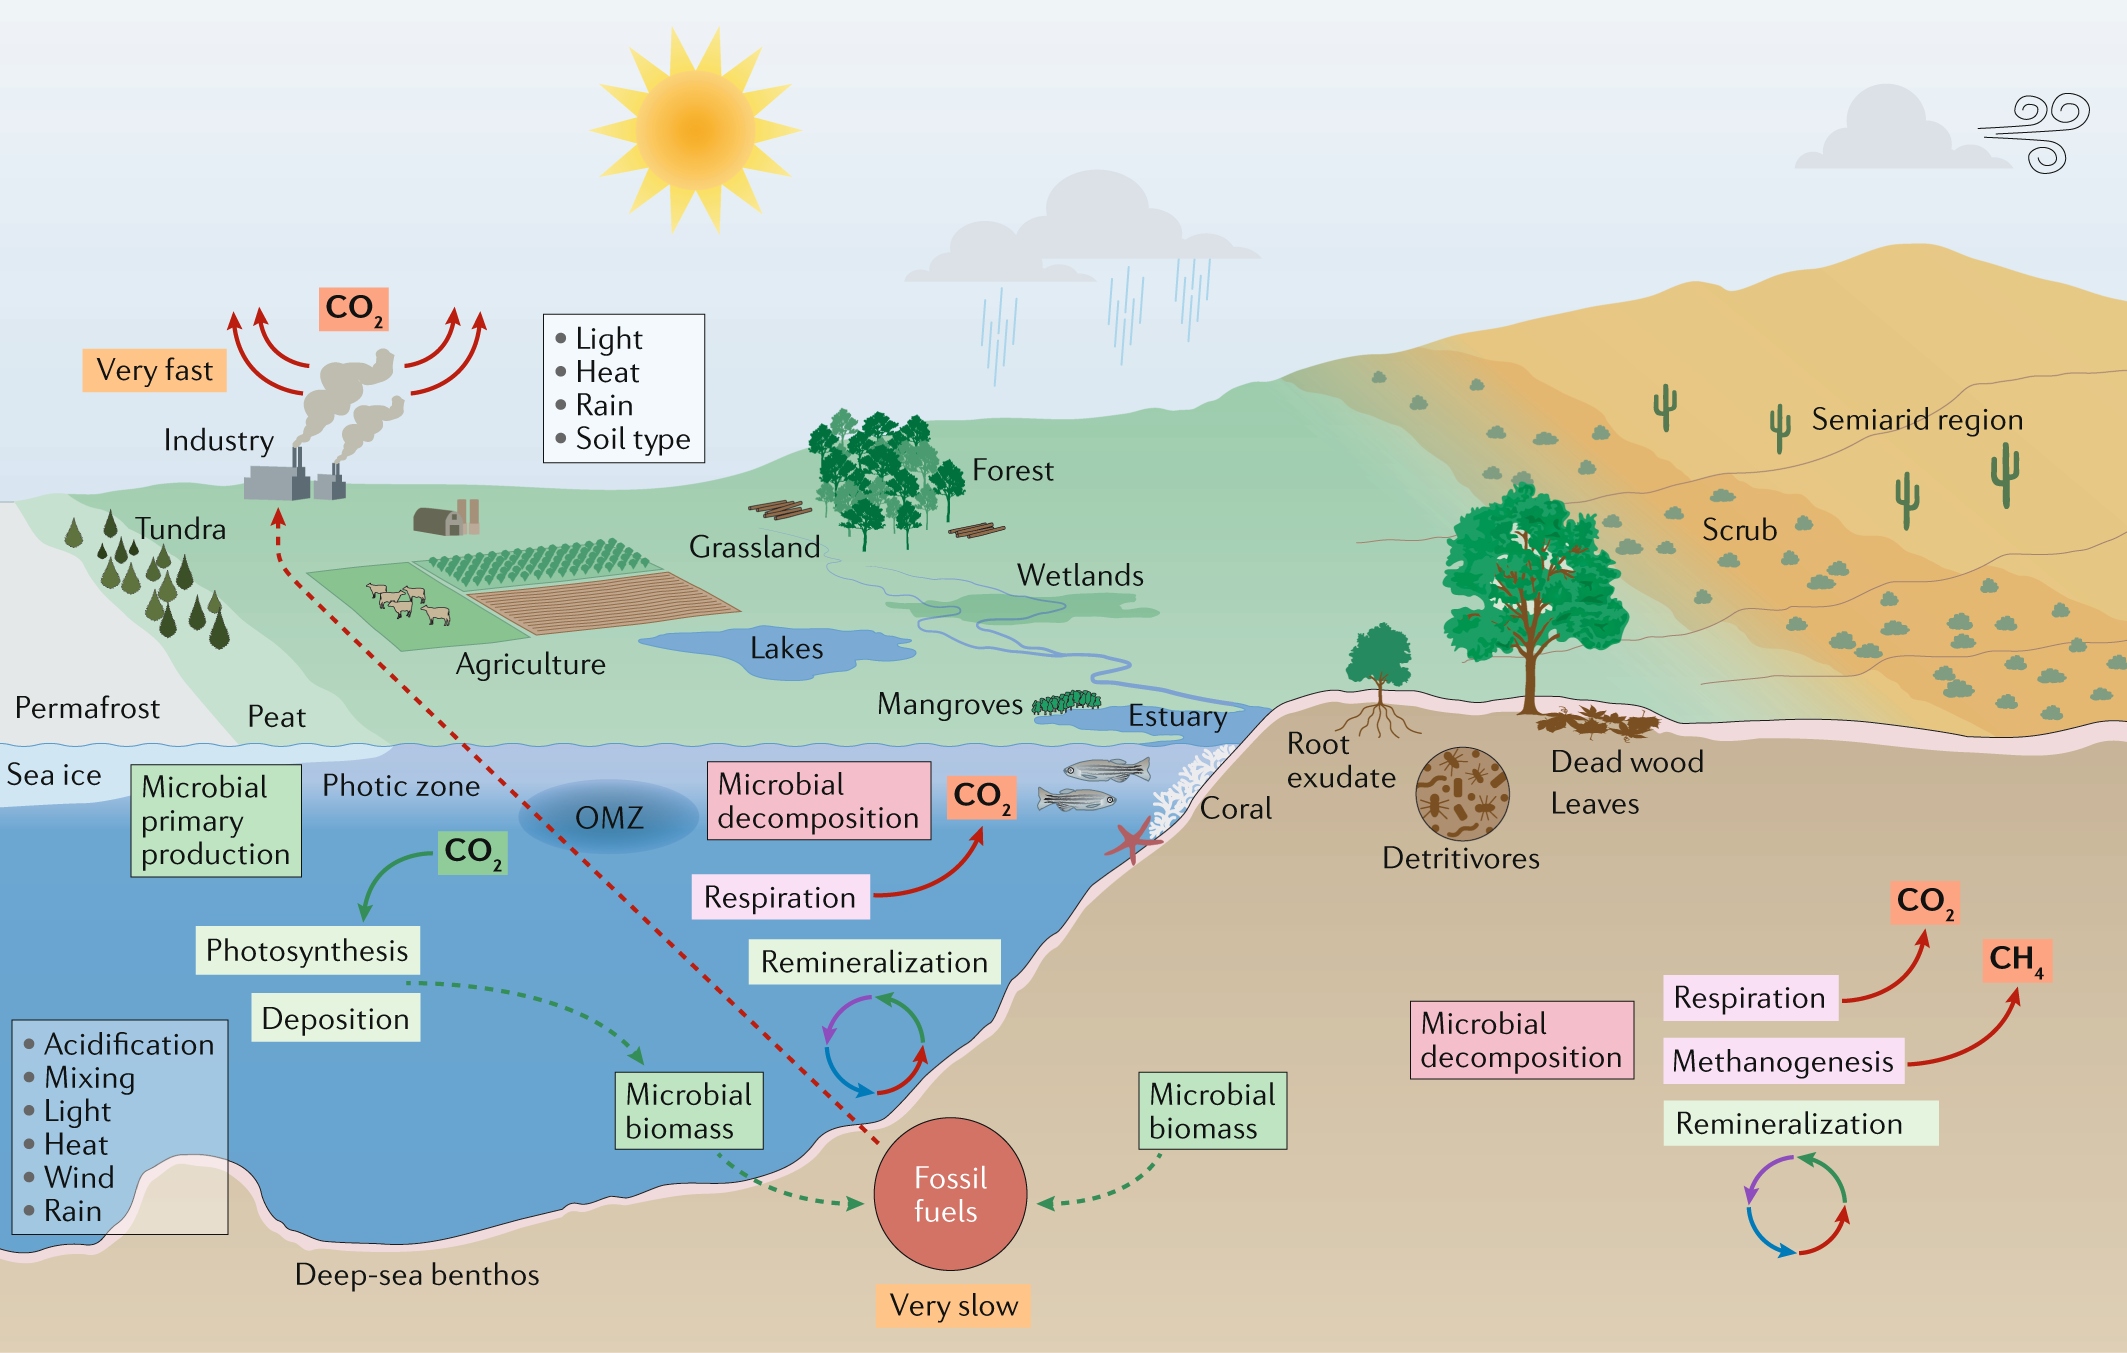
\includegraphics[width=85mm]{resources/ecosystem_functioning.png}
         \caption{
            \scriptsize Figure from: Cavicchioli et al.
            \scriptsize Nature Reviews Microbiology 17.9 (2019): 569-586.
         }
      \end{figure}
   \end{frame}

   % MAIN QUESTIONS 
   \begin{frame}
      \frametitle{Questions to address}
      \framesubtitle{for a deeper understanding of microbial assemblages}
      \begin{singlespace}


         \begin{columns}[onlytextwidth]
            
            \column{.33\textwidth}

               \begin{center}

                  Community \\ structure   \\ \textbf{\textit{who}}  

                  \hrulefill

                  \scriptsize \textit{eveyrone is everywhere}

               \end{center}


            \column{.33\textwidth}

               \begin{center}

                  Functional \\ potential \\ \textbf{\textit{what}}

                  \hrulefill

                  \scriptsize \textit{zero-sum game}

               \end{center}

            \column{.33\textwidth}

               \begin{center}

                  Microbial \\ interactions \\ \textbf{\textit{why}}

                  \hrulefill

                  \scriptsize \textit{the entagnled bank}

               \end{center}
      

         \end{columns}

      \end{singlespace}

   \end{frame}

   % BIOINFORMATICS 
   \begin{frame}

      \frametitle{We are living in a computational era}
      \framesubtitle{both a challenge \& an opportunity}

      
\includegraphics[width=85mm]{resources/bioinfo_transparent.png}

   \end{frame}



   % -------------------------
   % CHANGE THE CHAPTER SLIDE: HIGH THROUGHPUT SEQUENCING INTRO
   % -------------------------

   \begin{darkframes}
      \section{
         Bioinformatics methods for microbial diversity assessment
      }
   
   \end{darkframes}

   % MARKER GENES - BIOINFO STEPS
   \begin{frame}
      
      \frametitle{eDNA metabarcoding}
      \framesubtitle{for biodiversity assessment}
      \begin{singlespace}


         \begin{columns}[onlytextwidth]

            \column{.5\textwidth}

               \textbf{Marker genes} \\ 

               \begin{enumerate}
                  \item \textbf{16S rRNA:} Bacteria, Archaea
                  \item \textbf{12S rRNA:} Vertebrates
                  \item \textbf{18S rRNA:} Small eukaryotes, Metazoa
                  \item \textbf{ITS:} Fungi
                  \item \textbf{COI:} Eukaryotes
                  \item \textbf{\textit{rbcl}:} Plants
                  \item \textbf{\textit{dsrb}:} Bacteria, Archaea
                  \item ...
               \end{enumerate}

            \column{.45\textwidth}

               \textbf{Methodology}

               \begin{figure}
                  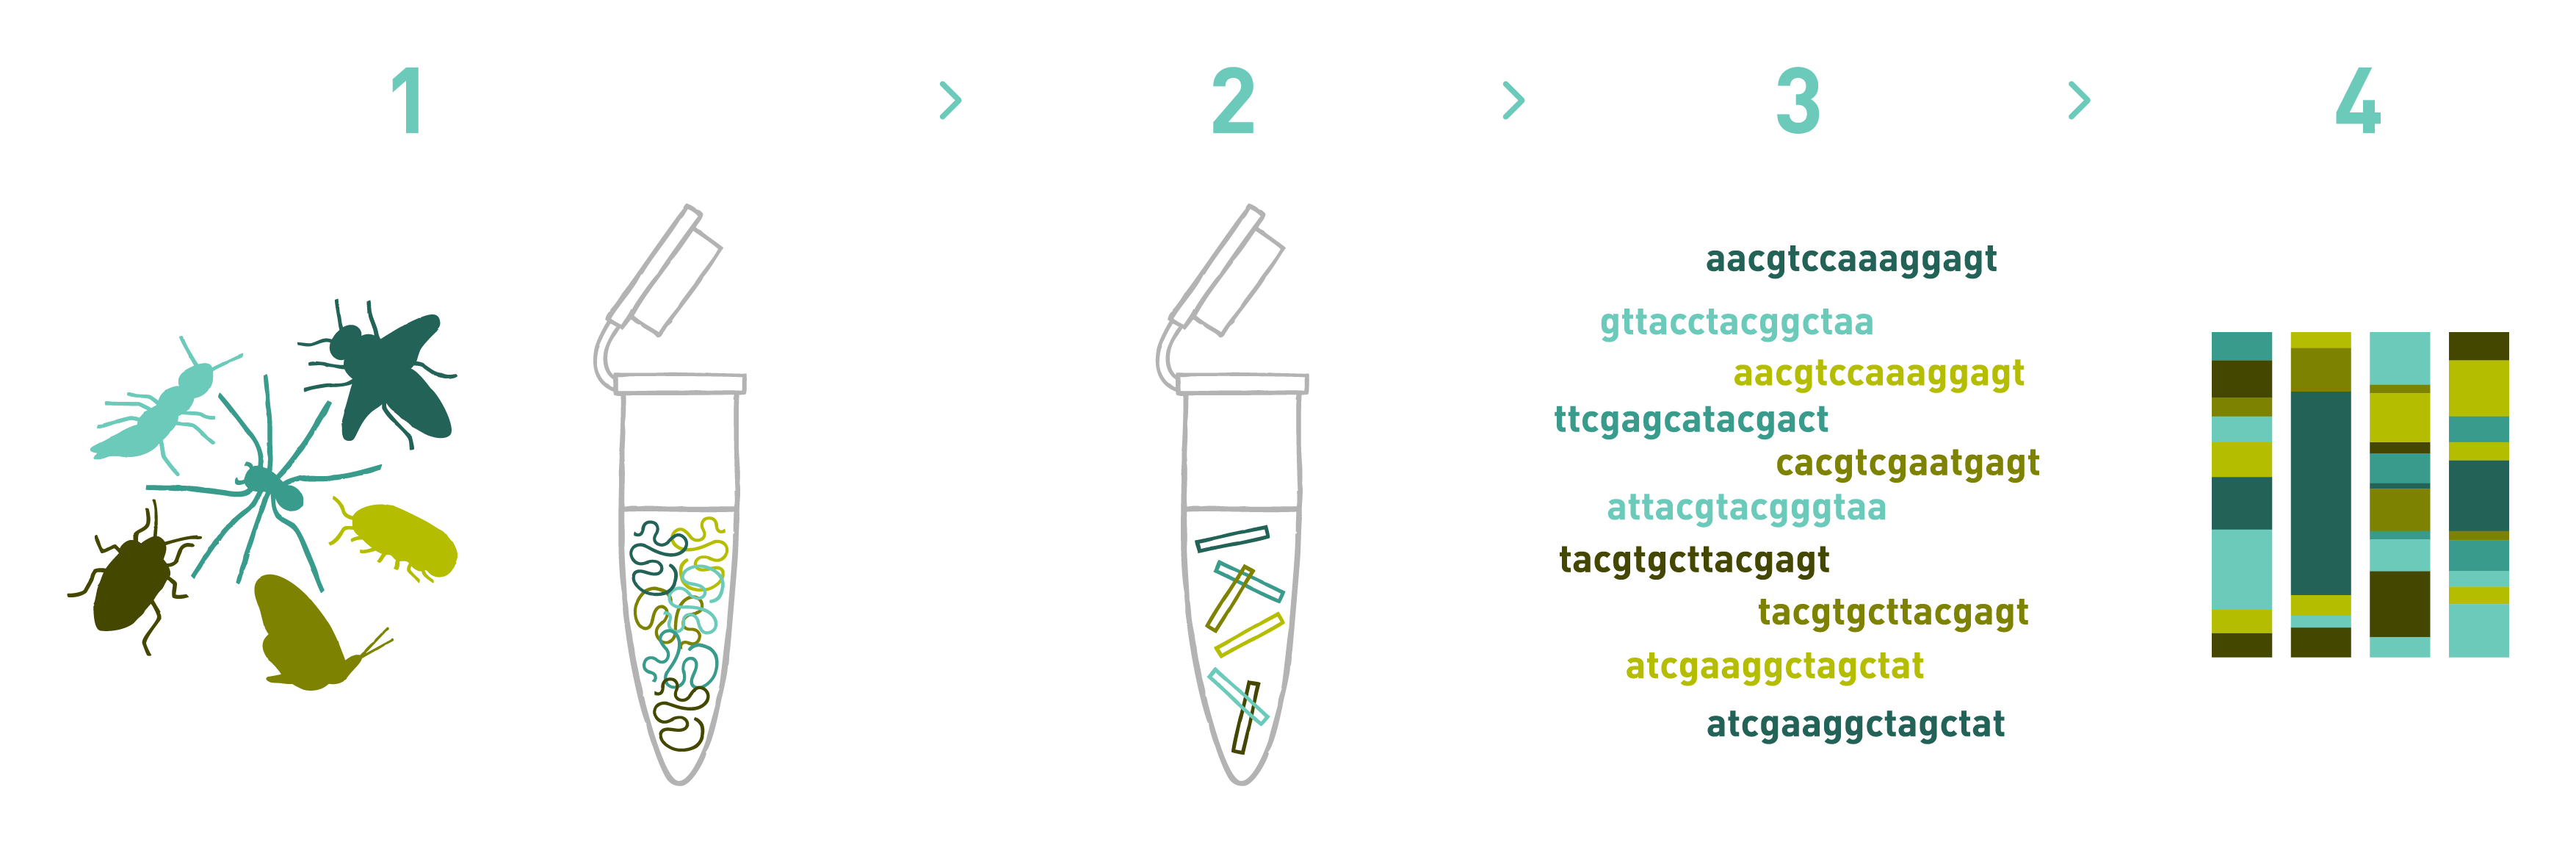
\includegraphics[width=55mm]{resources/metabarcoding-steps.png}
               \end{figure}

               \begin{itemize}
                  \item Sampling
                  \item Extraction
                  \item Bioinformatics
                  \item Biodiversity analysis
               \end{itemize}
               

         \end{columns}

      \end{singlespace}
   \end{frame}

   % BIOINFORMATICS CHALLENGES 
   \begin{frame}
      \frametitle{Bioinformatics challenges}
      \framesubtitle{for the analysis and the interpretation of amplicon data}

      \begin{columns}[onlytextwidth]

         \column{.5\textwidth}

            
\includegraphics[width=40mm]{resources/bioinfo_mess.png}



         \column{.5\textwidth}

            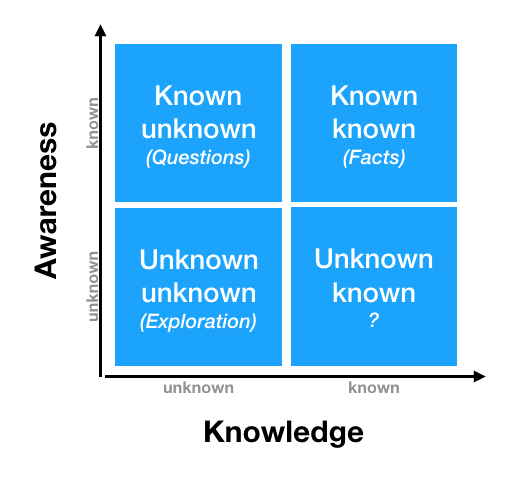
\includegraphics[width=50mm]{resources/known_unknown.png}
         
      \end{columns}
   \end{frame}


   % -------------------------
   % CHANGE SUBSECTION: PEMA 
   % -------------------------

   % BRIDGE SLIDE
   \begin{darkframes}

      \subsection{\texttt{pema}: a metabarcoding pipeline}

      % PEMA LOGO
      \begin{frame}

         \begin{figure}
            \centering
            
\includegraphics[width=60mm]{resources/pema_logo.png}         
         \end{figure} 

         \begin{textblock*}{7cm}(3.5cm, 8.2cm)
            \href{https://github.com/hariszaf/pema}{https://github.com/hariszaf/pema} \\ 
            \href{http://pema.hcmr.gr}{pema.hcmr.gr}
         \end{textblock*}


      \end{frame}

   \end{darkframes}

   % WORKFLOW SLIDE
   \begin{frame}
      \frametitle{PEMA features}
      \framesubtitle{one step at a time!}
      \begin{singlespace}
         \begin{tikzpicture}[overlay,remember picture]
            \node[anchor=west, xshift=30pt,yshift=-165pt]
               at (current page.north west) {
                  \includegraphics[width=104mm]{resources/pema-pema.drawio.png}
               };

         \end{tikzpicture}
      \end{singlespace}
   \end{frame}

   % BIOINFORMATICS TRICKS AND HINTS
   \begin{frame}
      \frametitle{PEMA coding insights}
      \framesubtitle{Being a \texttt{geek} just for a bit !}

      \begin{columns}[onlytextwidth]
         
         \column{0.5\textwidth}
         
            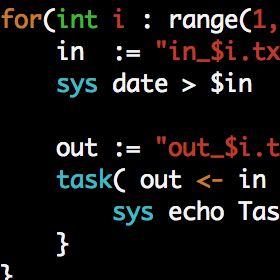
\includegraphics[width=25mm]{resources/bds.png}

            \texttt{BigDataScript} \\
            programming language

         \column{0.5\textwidth}

            \begin{tikzpicture}[overlay,remember picture]

               \node[anchor=east, xshift=-130pt, yshift=10pt]               
                  at (current page.east) {

                     
\includegraphics[width=20mm]{resources/sing_transp.png}
                  
                  };

                  \node[anchor=east, xshift=-40pt, yshift=10pt]
                  at (current page.east) {

                     
\includegraphics[width=25mm]{resources/docker_facebook_share.png}
                  
                  };

                  \node[anchor=south, align = center, above, xshift=60, yshift=90]
                  at (current page.south) {

                     Containerization

                  };

            \end{tikzpicture}
            
            % \bigskip
            % Containerization


      \end{columns}


   \end{frame}

   % INPUT - OUTPUT - RUN WITH A SINGLE COMMAND
   \begin{frame}

      \frametitle{Mount your I/O}
      \framesubtitle{give \& take}

      \begin{tikzpicture}[overlay,remember picture]

         \node[anchor=west, xshift=10pt, yshift=-10pt]               
            at (current page.west) {

               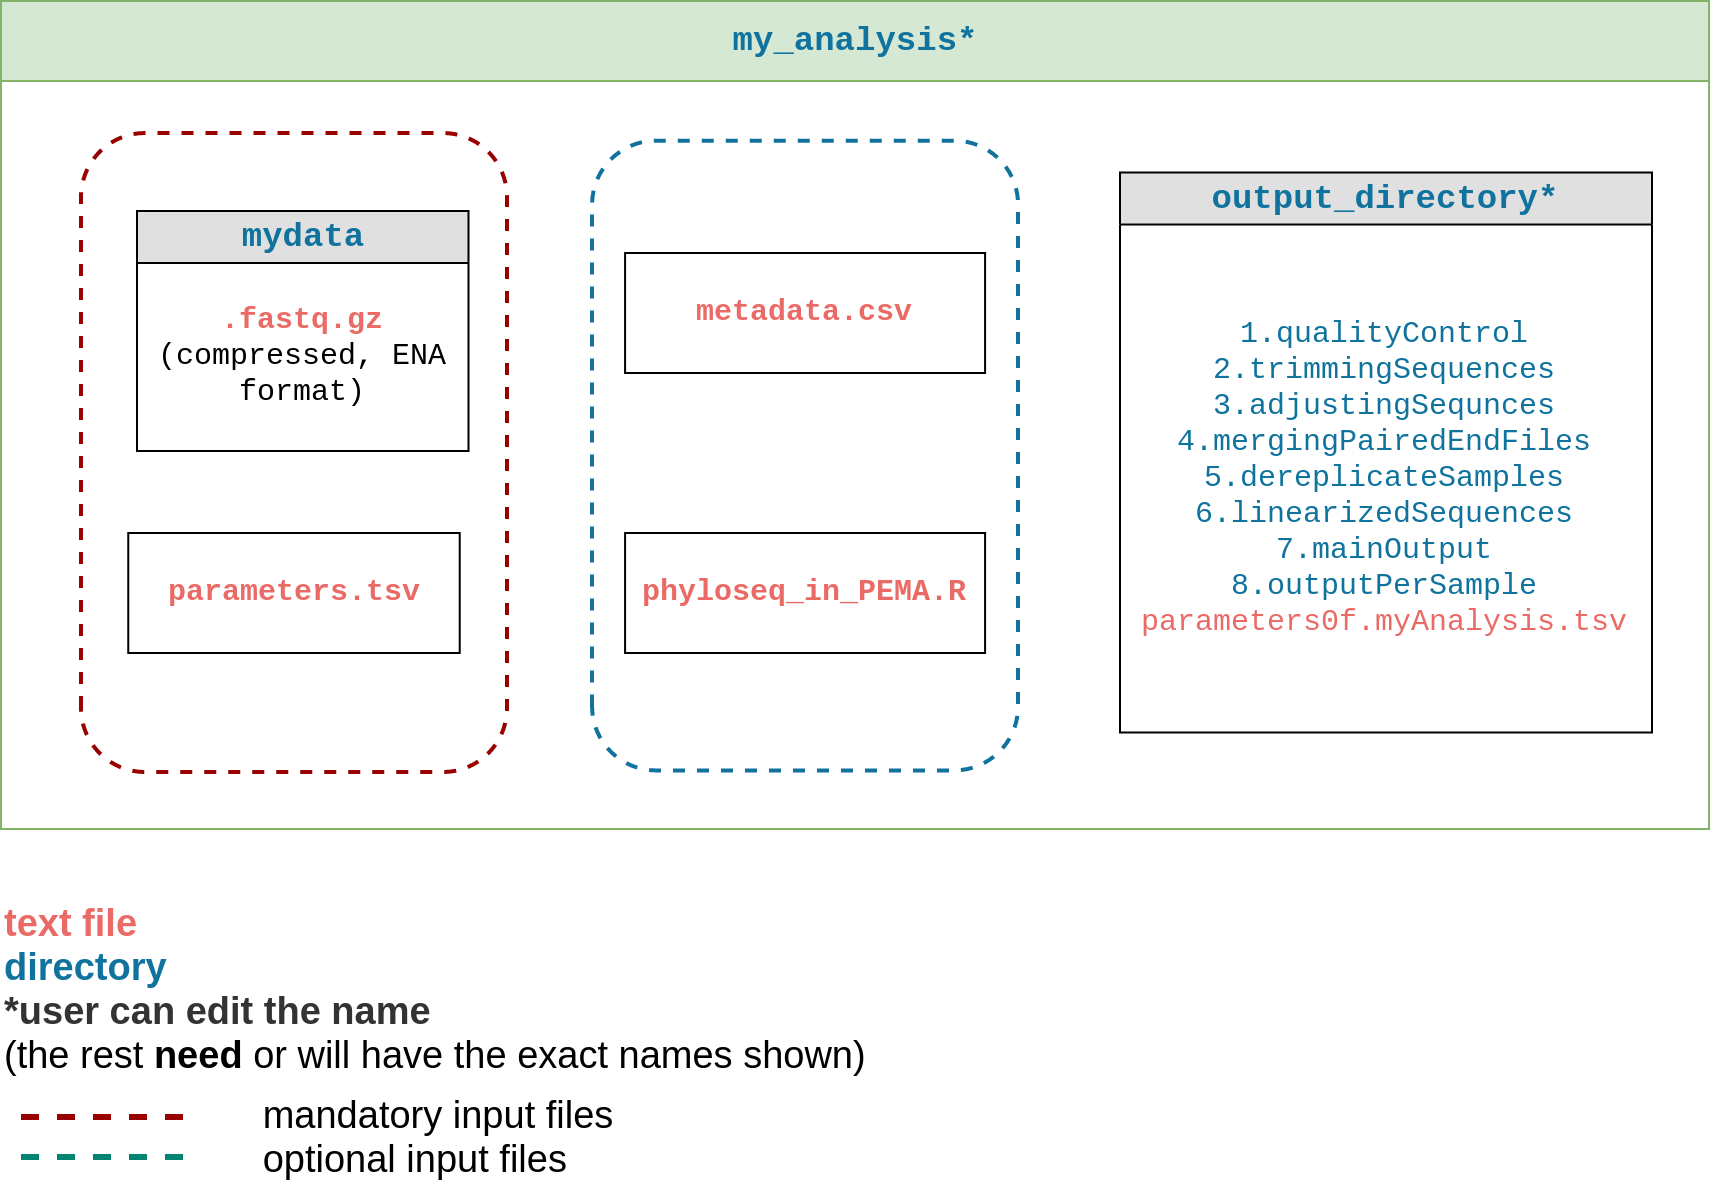
\includegraphics[width=75mm]{resources/pema_anlysis_dir-Page-1.drawio.png}
            
            };

         \node[anchor=east, xshift=-10pt, yshift=50pt]               
         at (current page.east) {

            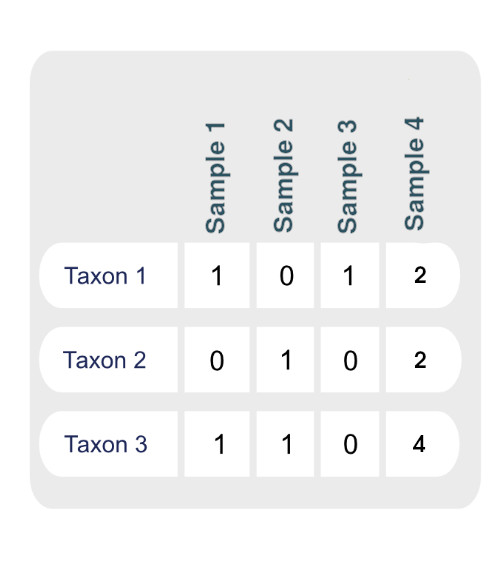
\includegraphics[width=35mm]{resources/final_table.jpg}
         
         };

         \node[anchor=east, xshift=-10pt, yshift=-60pt]
         at (current page.east) {

            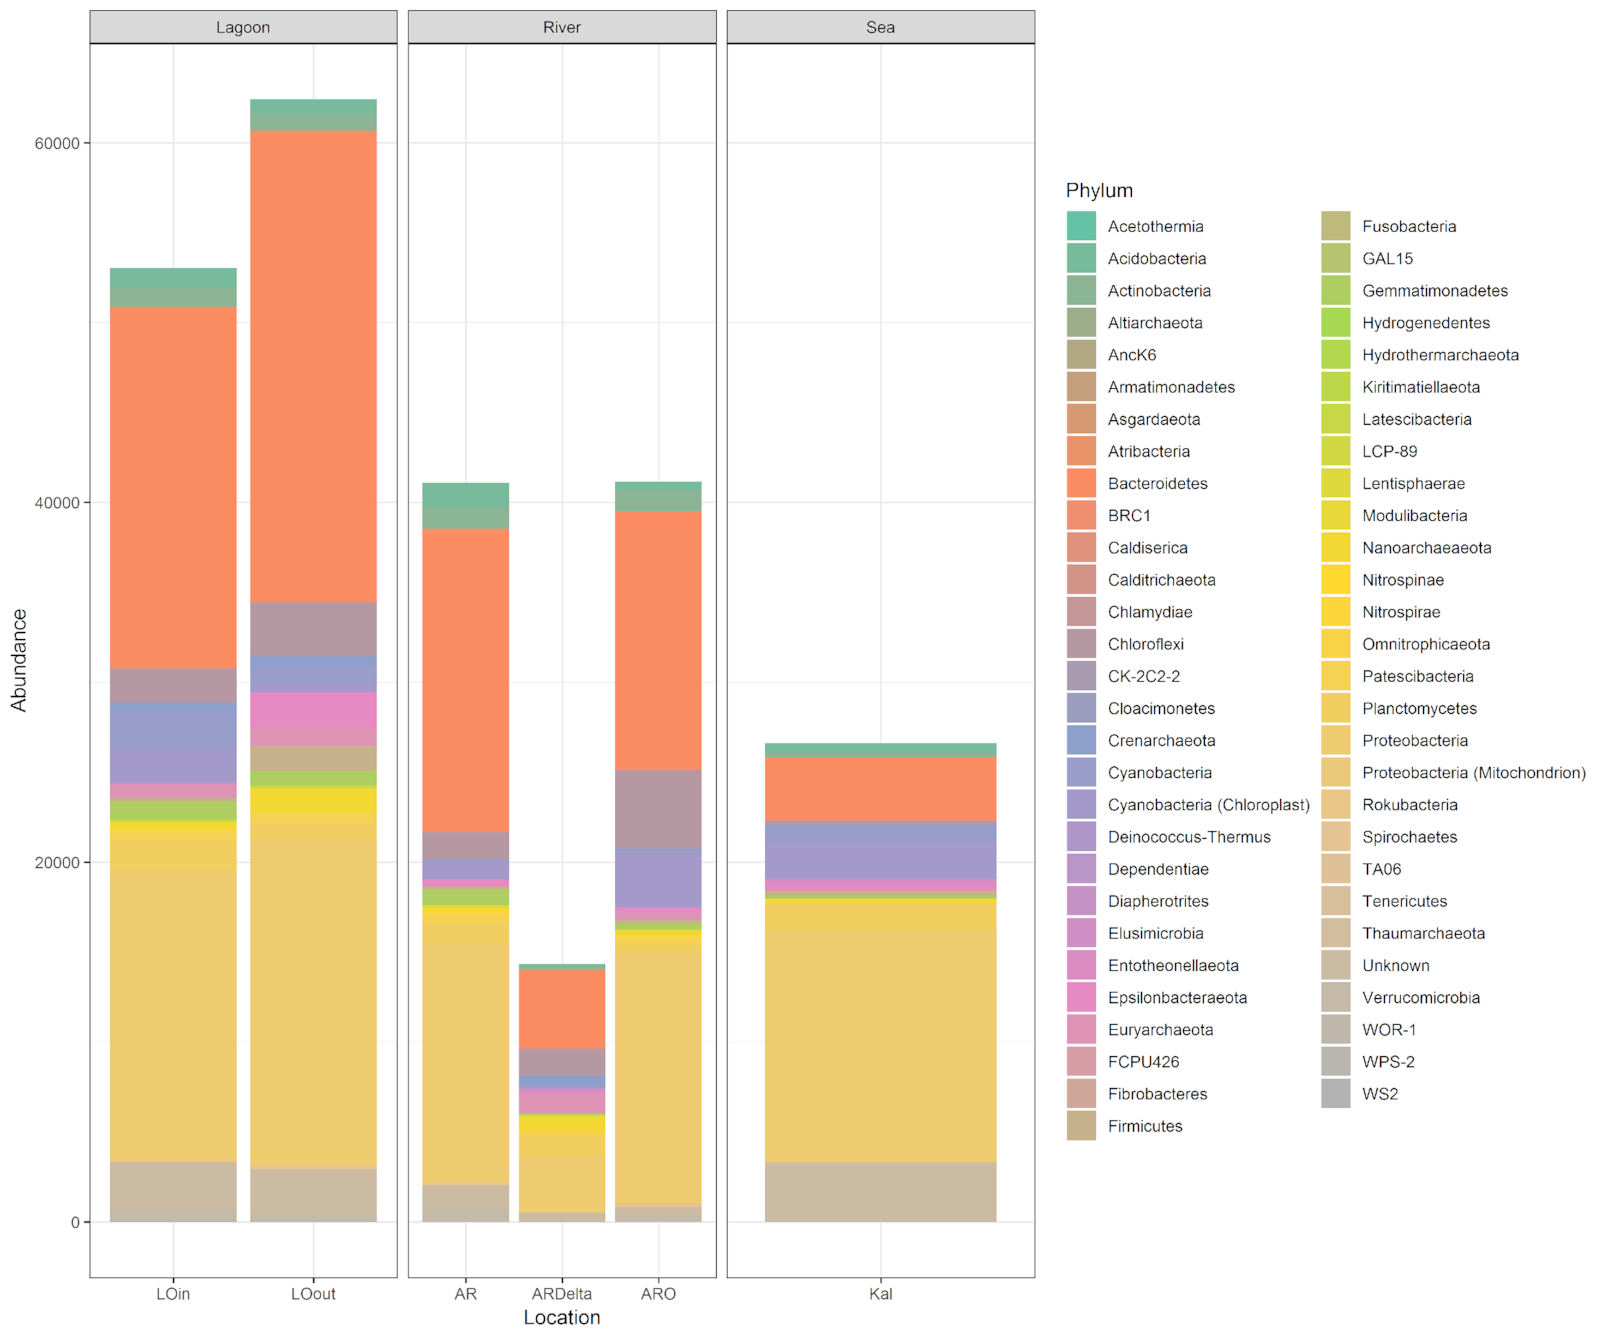
\includegraphics[width=43mm]{resources/giaa022fig3.jpeg}
         
         };


      \end{tikzpicture}
      
   
   \end{frame}

   % % PEMA PUBLICATION 
   % \begin{frame}
   %    \frametitle{PEMA publication}
   %    \framesubtitle{in 2020}
   %    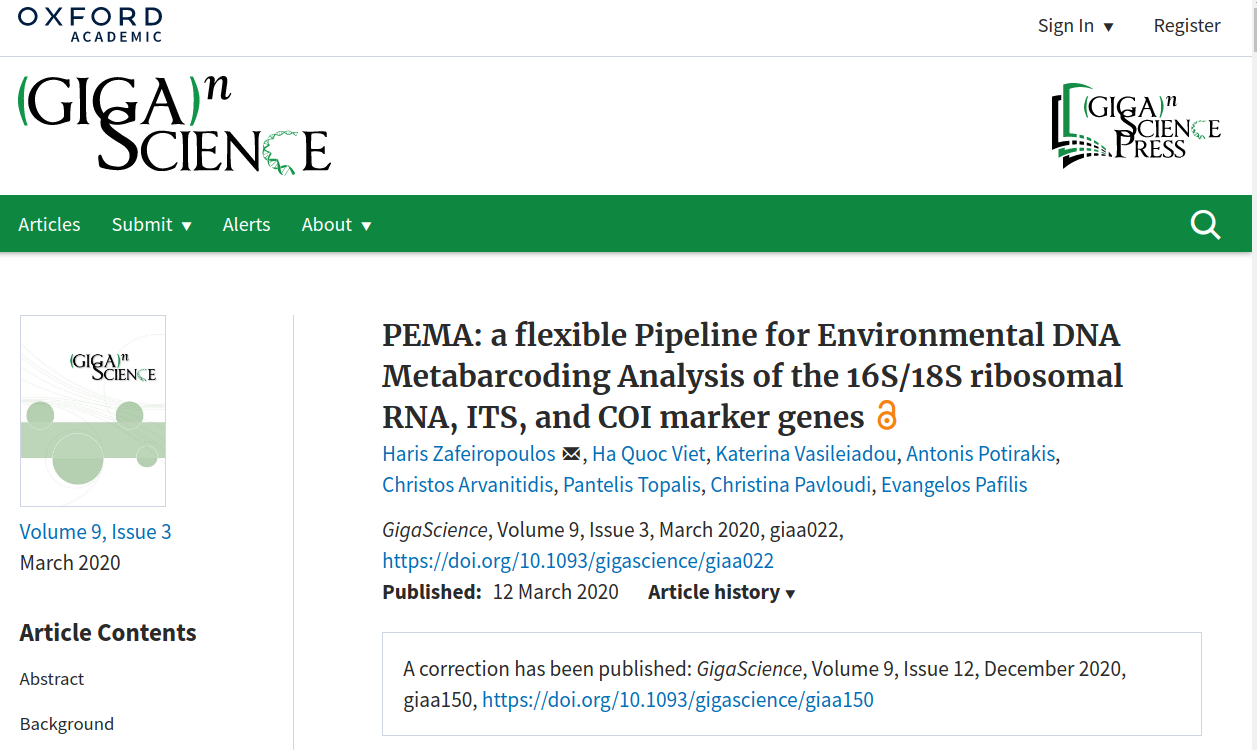
\includegraphics[width=100mm]{resources/pema_publ.png}
   % \end{frame}

   % WORKFLOW OF VERSION 2
   \begin{frame}
      \frametitle{PEMA v.2}
      \framesubtitle{addressing some of the challenges}

      \begin{singlespace}
         \begin{tikzpicture}[overlay,remember picture]
       
               \node[anchor=west, xshift=30pt,yshift=-150pt]
                  at (current page.north west) {
                     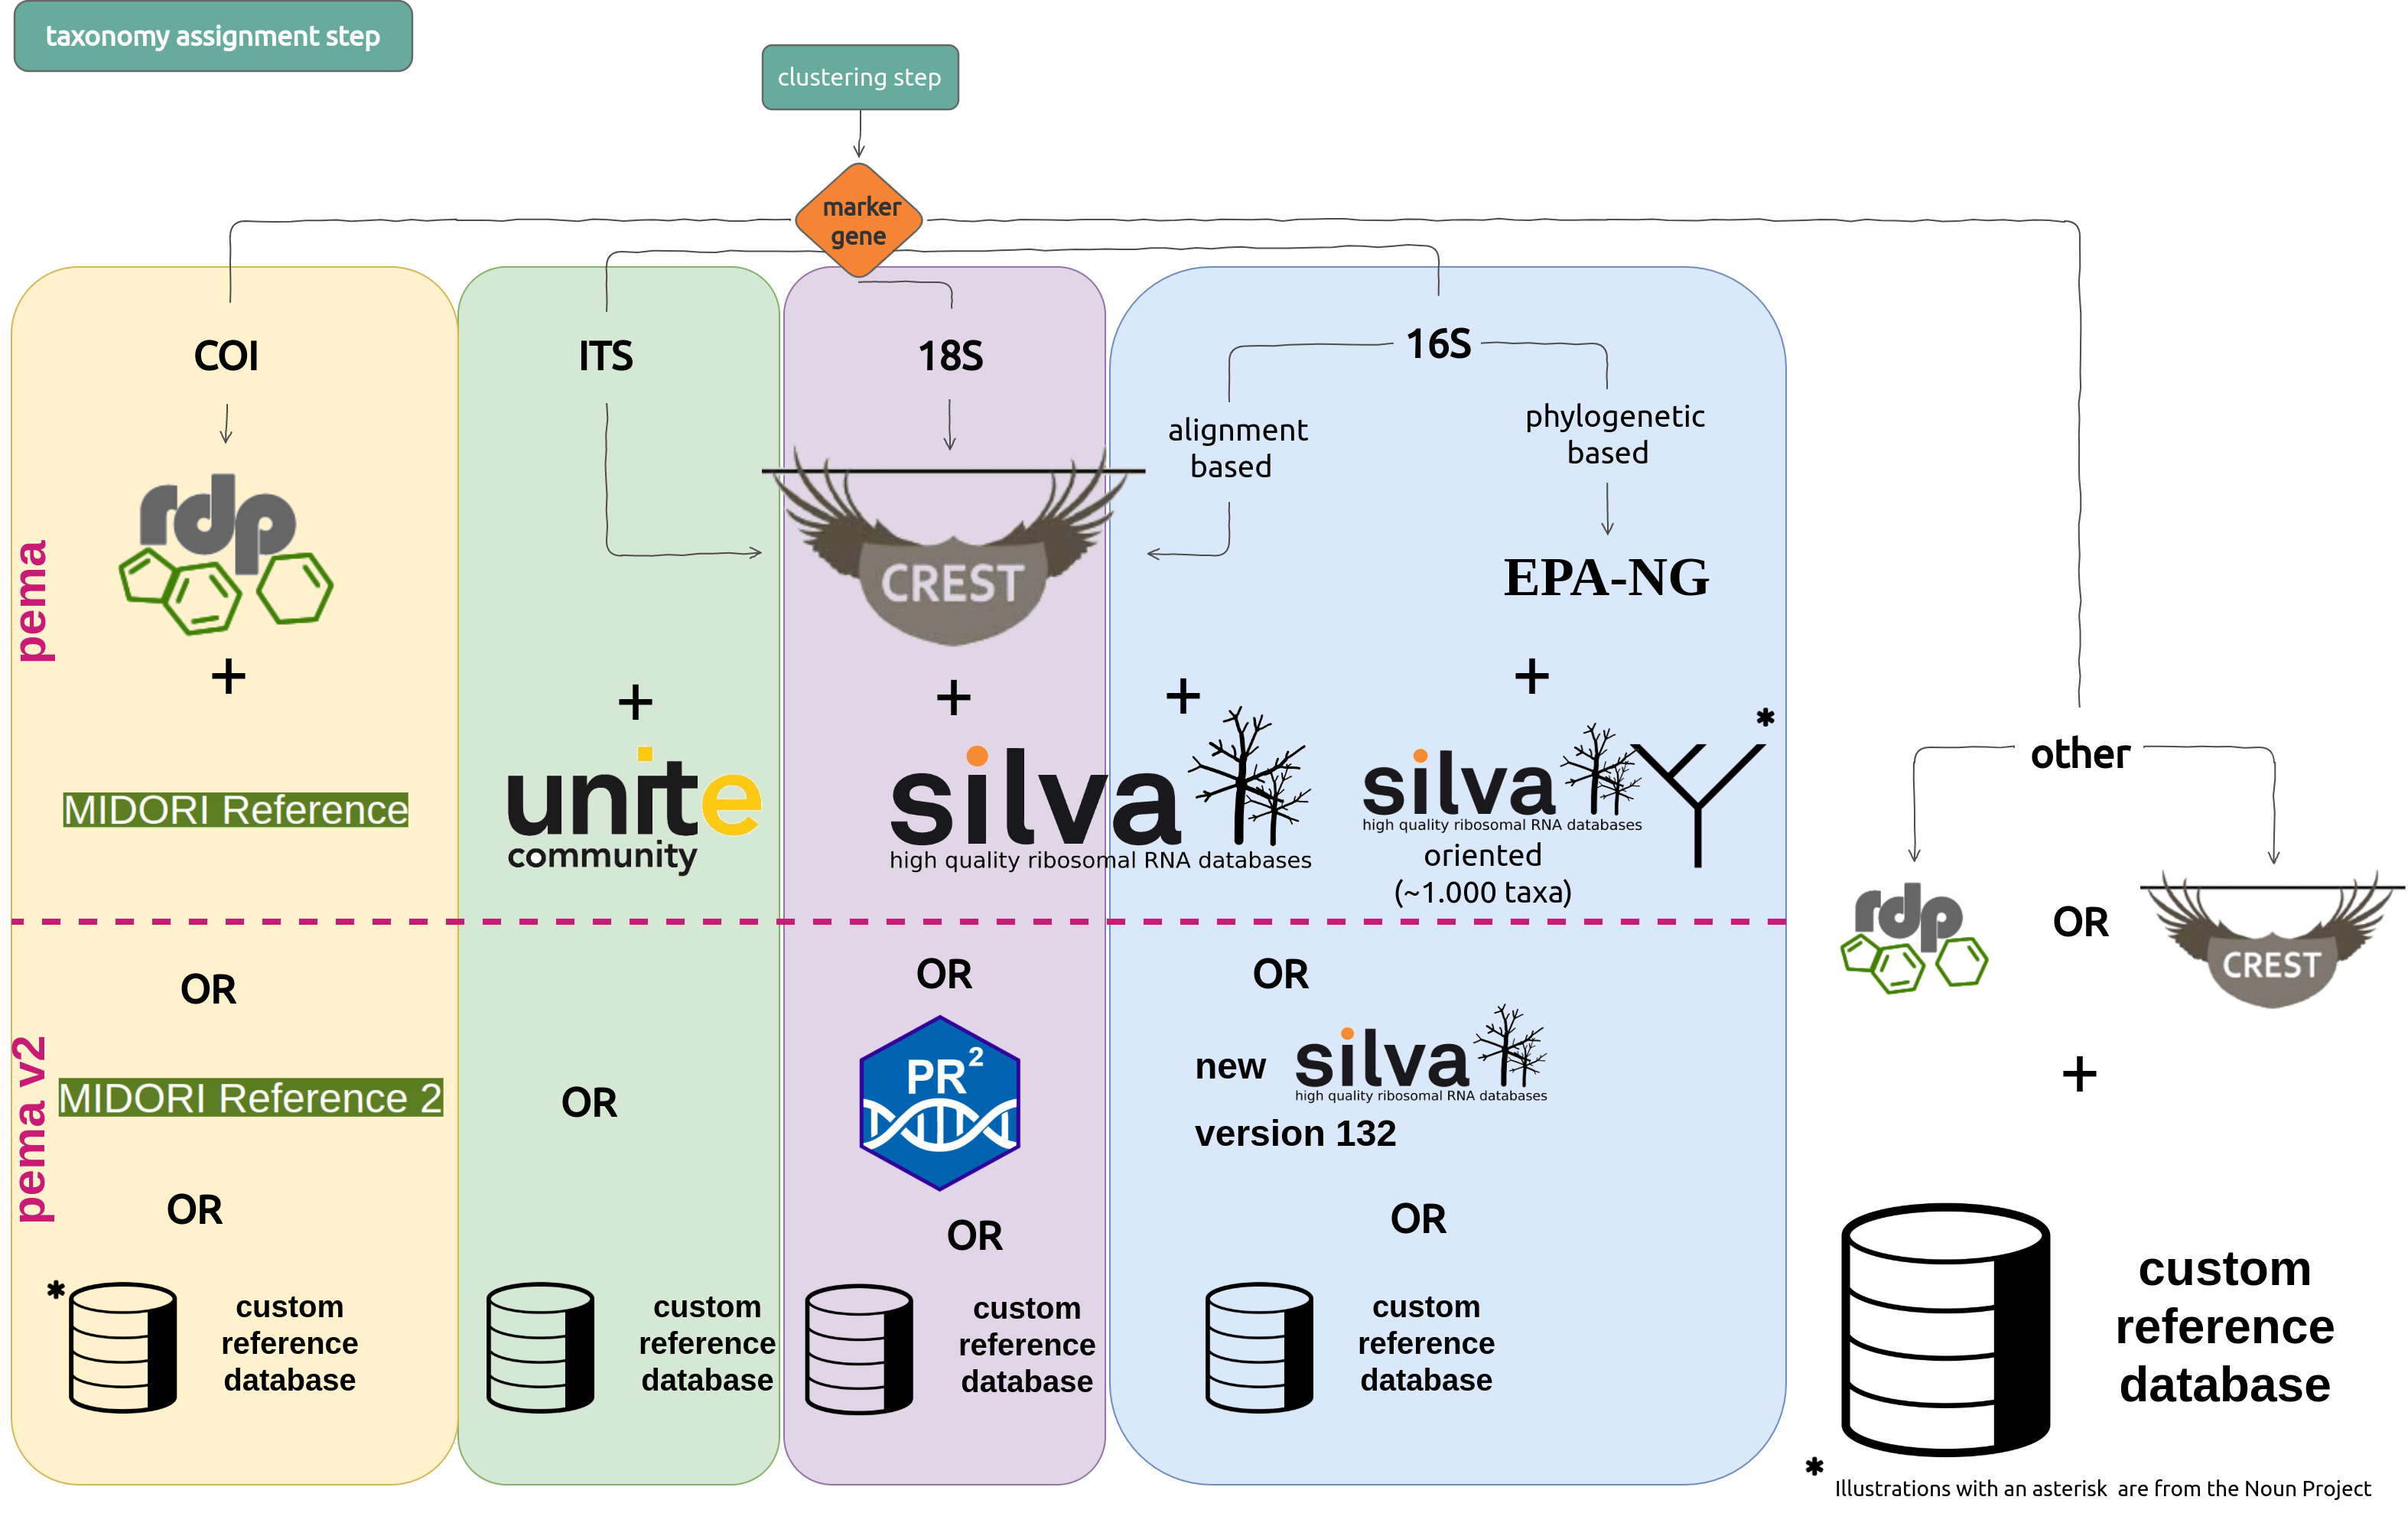
\includegraphics[width=100mm]{resources/pema-pema.v2.drawio.png}
                  };
                  
         \end{tikzpicture}

         \begin{textblock*}{5cm}(8.2cm, 2.3cm) % {block width} (coords) 
            
            \scriptsize Code architecture from scratch!

         \end{textblock*}

      \end{singlespace}
   \end{frame}

   % PEMA v.2.1.4 - ARMS
   \begin{frame}
      \frametitle{Latest PEMA version}
      \framesubtitle{addressing the challenges of the community}

      \begin{singlespace}
         \begin{tikzpicture}[overlay,remember picture]
       
               \node[anchor=west, xshift=30pt,yshift=-150pt]
                  at (current page.north west) {
                     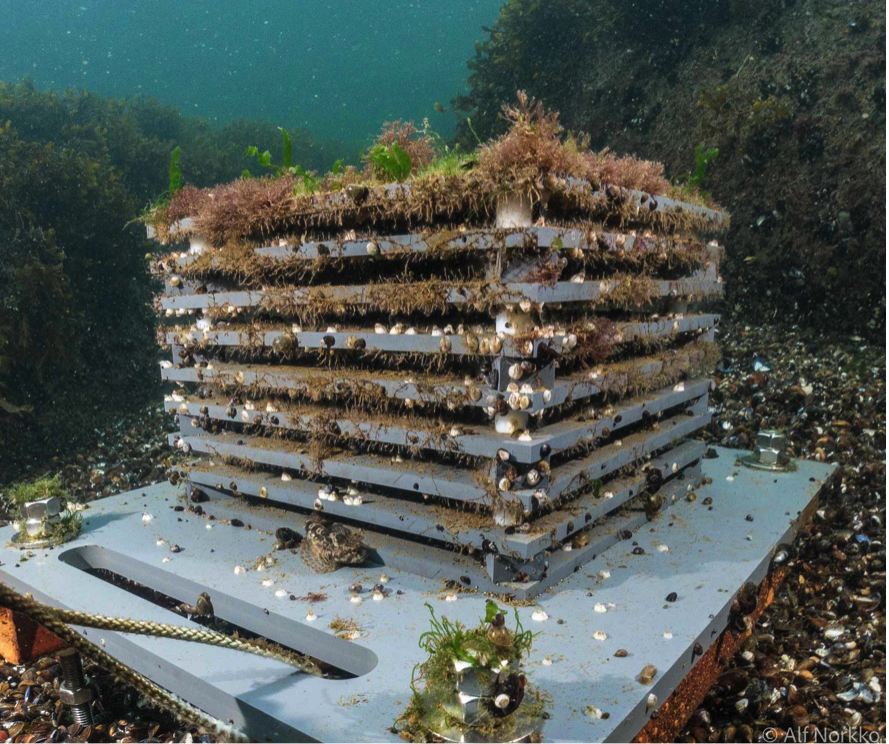
\includegraphics[width=55mm]{resources/Autonomous-Reef-Monitoring.png}
               };

               \node[anchor=east, xshift=-65pt,yshift=50pt]
                  at (current page.east) {
                     
\includegraphics[width=34mm]{resources/assemble_logo.png}
               };

               \node[anchor=east, xshift=-5pt,yshift=50pt]
                  at (current page.east) {
                     
\includegraphics[width=17mm]{resources/MBON_logo_transparent.png}

               };

         \end{tikzpicture}


         \begin{textblock*}{5cm}(7.2cm,4.0cm) % {block width} (coords) 
            
            \scriptsize

            \textbf{\texttt{pema:v.2.1.4} includes:}

            \begin{enumerate}
               \item analysis of 12S rRNA data now supported
                     (\href{https://github.com/terrimporter/12SvertebrateClassifier/releases}{12S Vertebrate Classifier v2.0.0-ref} database) 
               \item PR2 as an alternative reference 
                     database for the case of 18S rRNA 
               \item the \texttt{ncbi-taxonomist} tool \\ 
                     was added to return the NCBI Taxonomy \\ 
                     Id of the taxonomies found
            \end{enumerate}

         \end{textblock*}


      \end{singlespace}
   \end{frame}

   % GitHub repo
   % \begin{frame}
   % \frametitle{open source is cool}
   %    \framesubtitle{interacting with the community}

   %    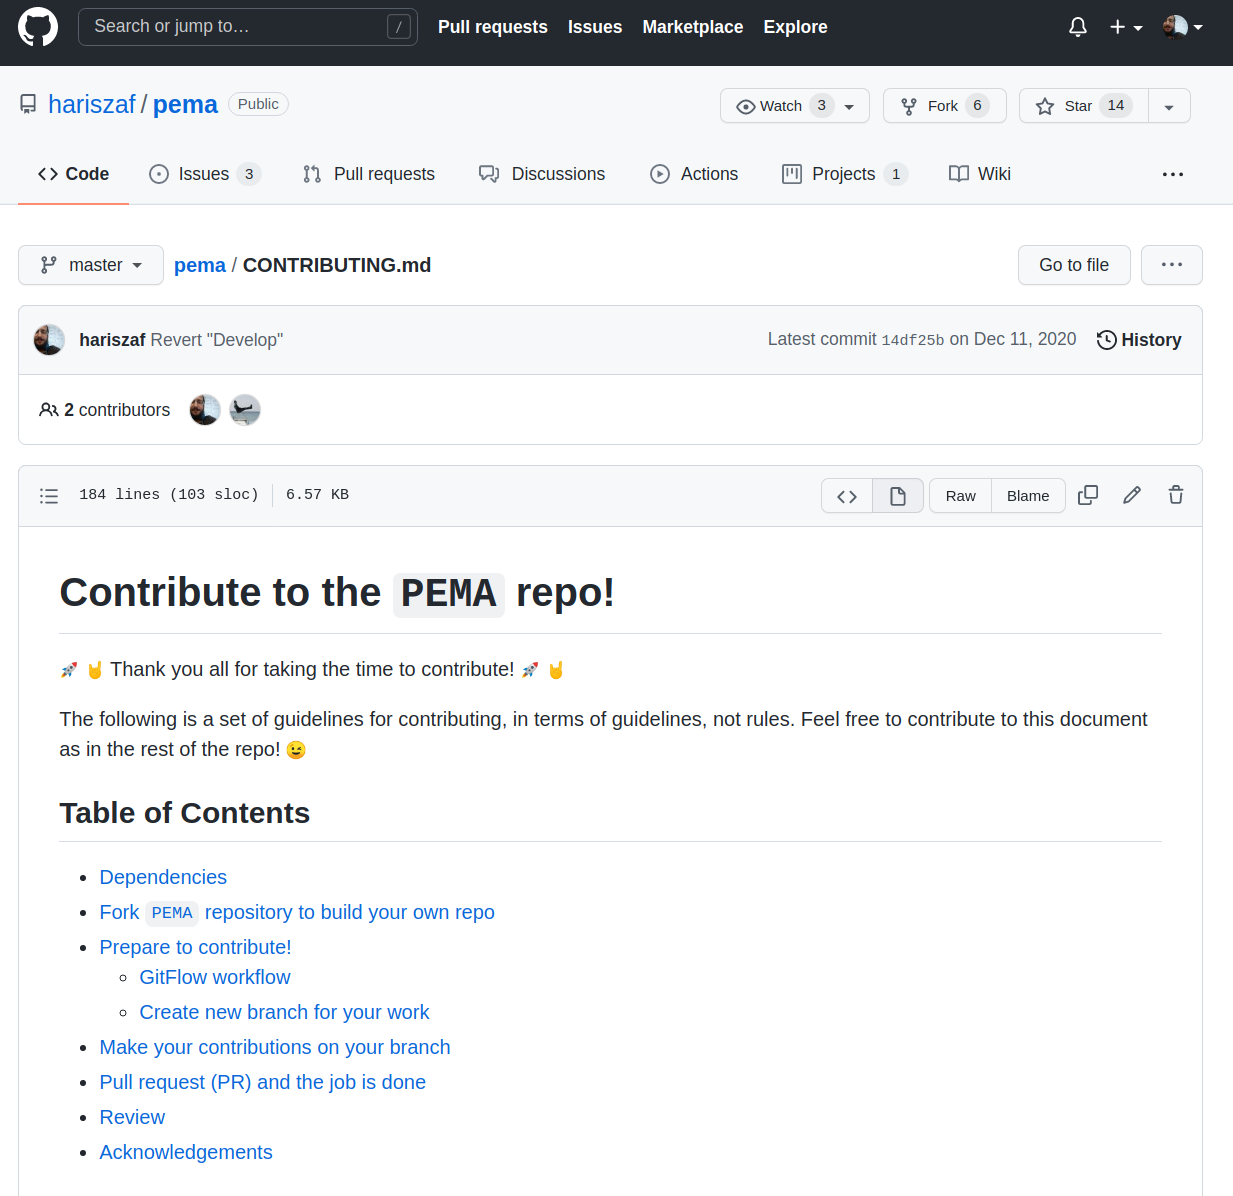
\includegraphics[width=60mm]{resources/pema_contribution.png}

   %    \small
   %    \begin{textblock*}{5cm}(7.5cm,4.0cm) % {block width} (coords) 
   %       PEMA aims at building a community 
   %       to discuss challenges on metabarcoding
   %       come up with solutions and why not 
   %       develop some of them! 
   %    \end{textblock*}

   % \end{frame}

   % % PEMA WEBSITE
   % \begin{frame}
   %    \frametitle{\textit{How to} and further documentation}
   %    \framesubtitle{at \href{http://pema.hcmr.gr}{pema.hcmr.gr}}
   %    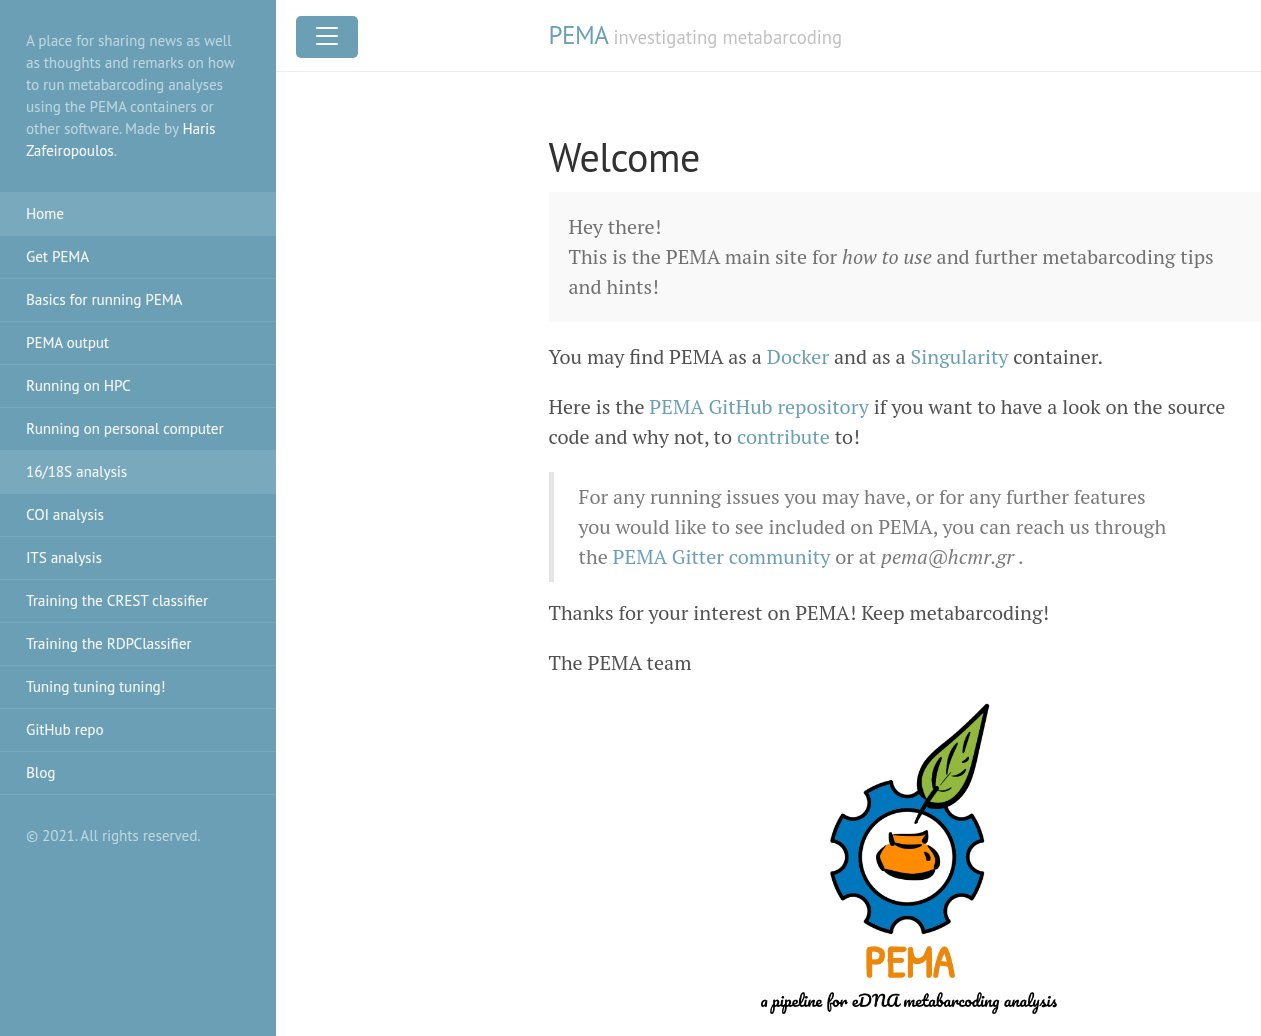
\includegraphics[width=85mm]{resources/pema_site.png}
   % \end{frame}



   % -------------------------------------
   % CHANGE SUBSECTION: DARN
   % -------------------------------------

   % DARN LOGO SLIDE
   \begin{darkframes}
      \subsection{\texttt{darn}: known unknowns in COI amplicon data}
      \begin{frame}
         \begin{figure}
            
\includegraphics[width=55mm]{resources/darn_logo.png}
            
\includegraphics[width=30mm]{../met_nets/resources/darn-logo-text.png}
         \end{figure}


         \begin{textblock*}{7cm}(3.5cm, 7.0cm)
            \href{https://github.com/hariszaf/darn}{https://github.com/hariszaf/darn}
         \end{textblock*}


      \end{frame}
   \end{darkframes}

   % DARN METHODOLOGY
   \begin{frame}
      \frametitle{Dark mAtteR iNvesigator}
      \framesubtitle{investigating known unknown \\ in COI amplicon data}

      \begin{textblock*}{7cm}(1.2cm, 4.5cm)
         What is all these unassigned  \\
         OTUs / ASVs? 
      \end{textblock*}

      \begin{singlespace}
         \begin{tikzpicture}[overlay,remember picture]
            \node[anchor=north east, xshift=-10pt,yshift=-5pt]
               at (current page.north east) {
                  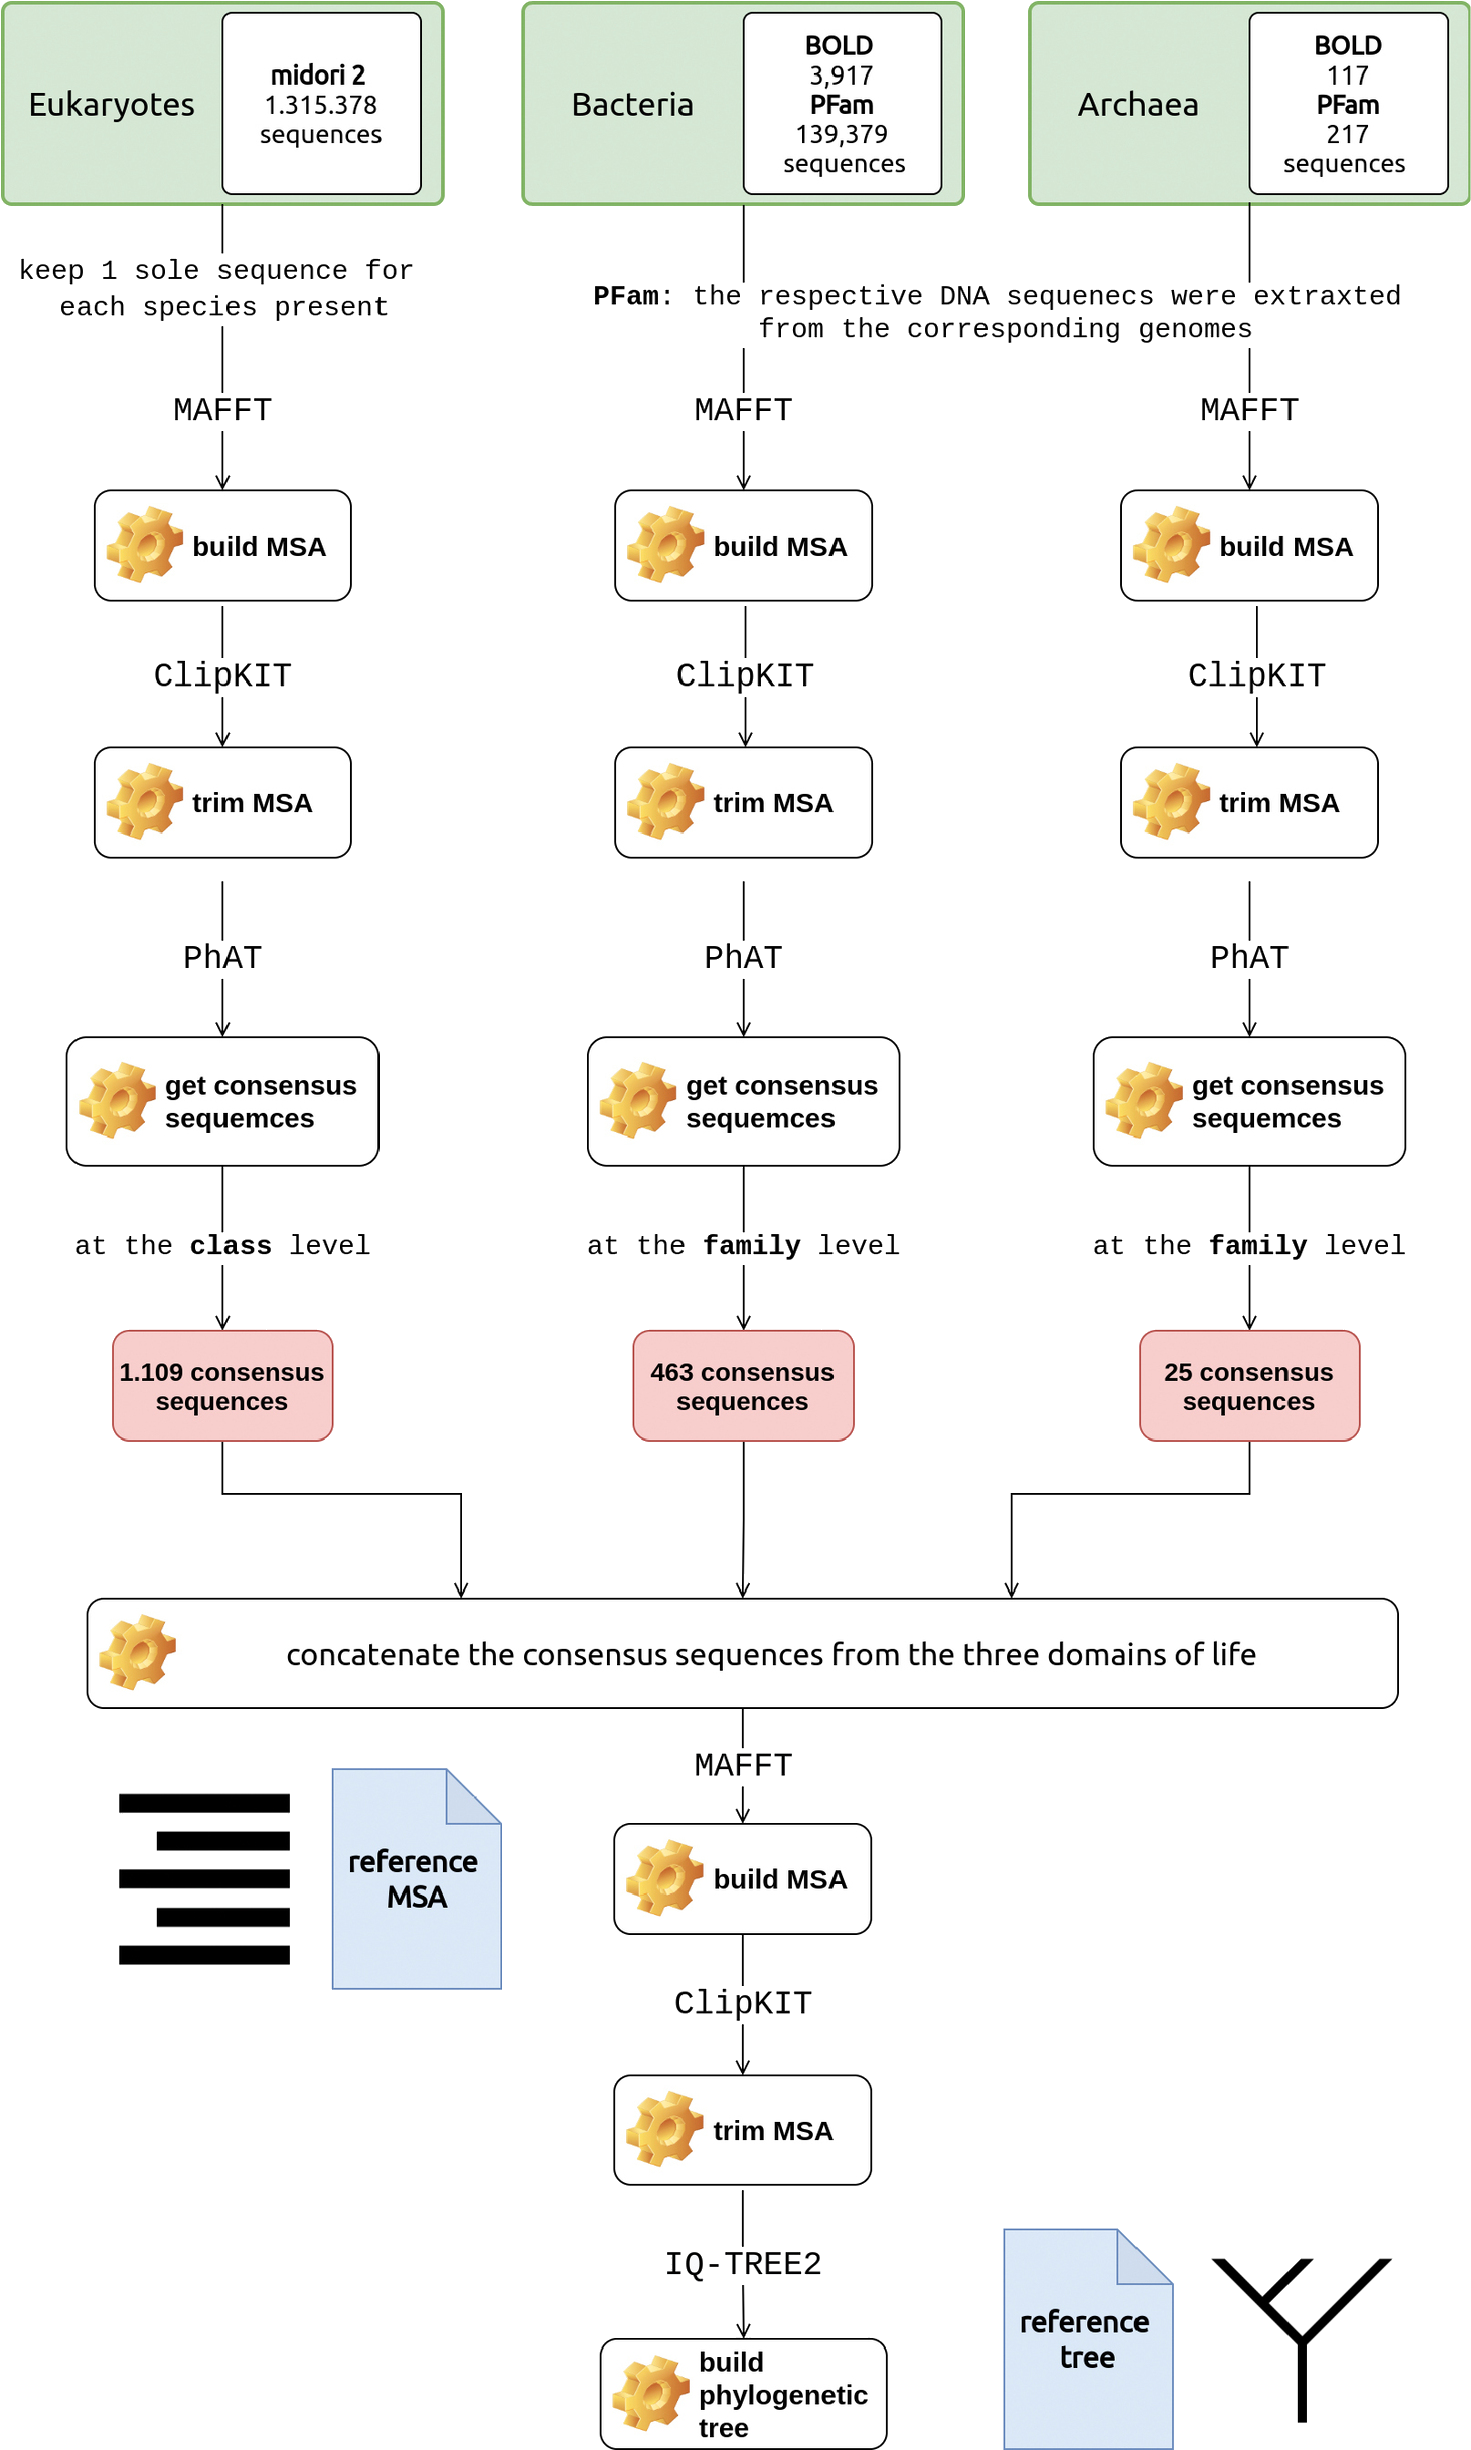
\includegraphics[width=50mm]{resources/darn_methodology_transparent.png}
               };
            \node[align = right, above, xshift=90, yshift=10] at (current page.south) {
               \scriptsize 
               Figure from: \href{https://doi.org/10.3897/mbmg.5.69657}{10.3897/mbmg.5.69657}
            };
         \end{tikzpicture}
      \end{singlespace}
   \end{frame}

   % DARN PHYLOGENY TREE
   \begin{frame}
      \frametitle{Phylogeny of the COI consensus sequences retrieved}
      \framesubtitle{the tree that DARN makes use of}
      \begin{tikzpicture}[overlay, remember picture]
         \node[anchor=west, xshift=10pt, yshift=-15pt]
         at (current page.west){
            \includegraphics[width=60mm]{resources/placements_of_consensus_seqs_transpaernt.png}
         };
      \end{tikzpicture}

      \begin{textblock*}{7cm}(7.0cm, 4.5cm)
         
         the consensus sequences have  \\ 
         been placed in their corresponding \\ 
         taxonomic branches, proving \\
         the tree valid

      \end{textblock*}
   \end{frame}

   % DARN OUTPUT
   \begin{frame}
      \frametitle{Bacteria are everywhere!}
      \framesubtitle{... Archaea too!}

      \begin{tikzpicture}[overlay, remember picture]
         \node[anchor=west, xshift=-20pt, yshift=2pt]
         at (current page.west){
            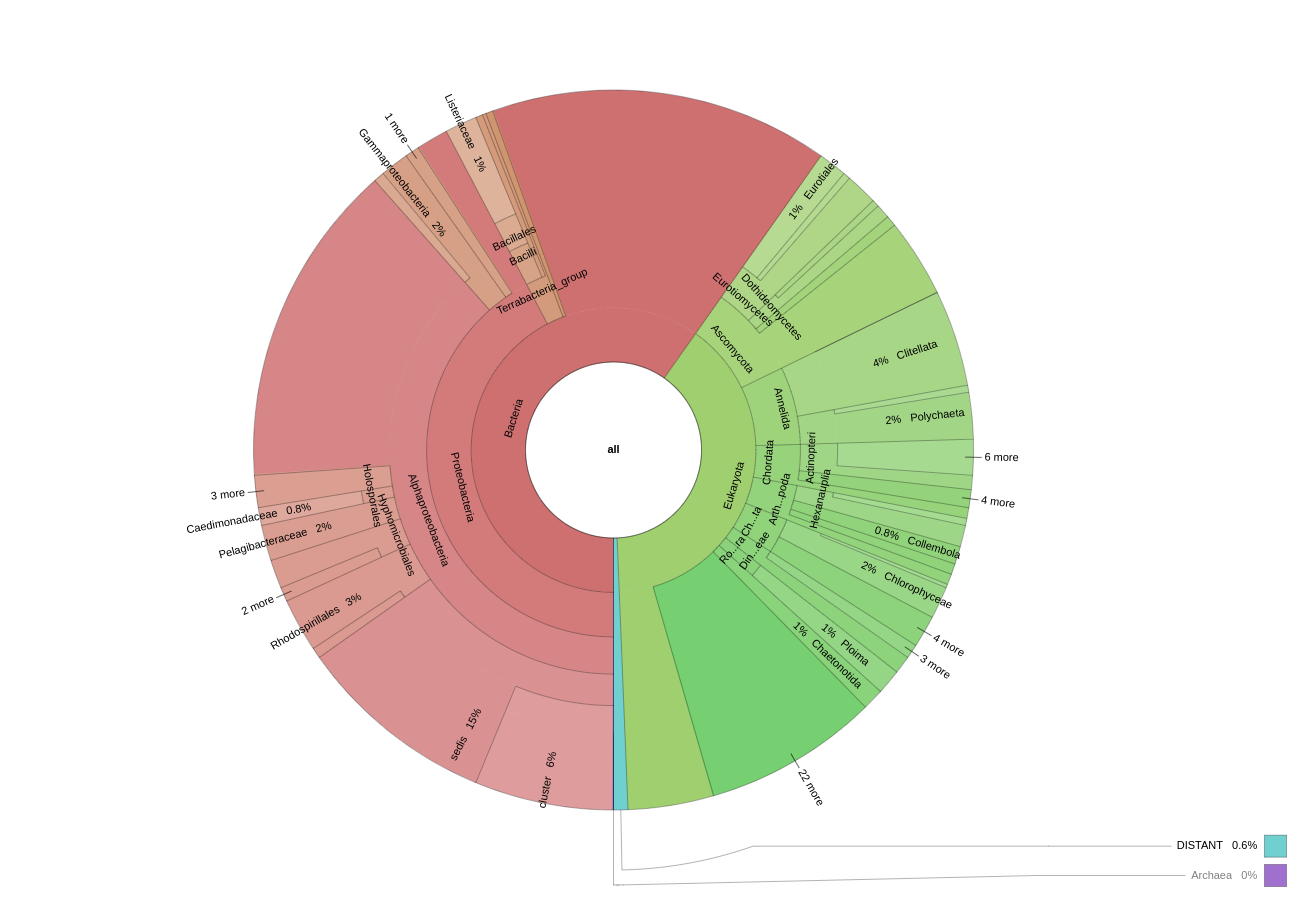
\includegraphics[width=90mm]{resources/darn_krona_output.png}
         };
      \end{tikzpicture}

      \begin{textblock*}{6cm}(7cm, 3.5cm)
         you may have a look at \\
         \href{https://hariszaf.github.io/darn/}{https://hariszaf.github.io/darn/} \\
         for more DARN output \\ 
         example cases
      \end{textblock*}

   \end{frame}


   % -------------------------------------
   % CHANGE THE CHAPTER SLIDE: PREGO
   % -------------------------------------

   \begin{darkframes}
      \section{
         \texttt{PREGO}: a knowledge-base for organisms - environments - processes associations
      }
   \end{darkframes}

   % PREGO LOGO - SLIDE
   \begin{frame}
      
      \begin{figure}
         
\includegraphics[width=75mm]{resources/prego_logo.png}
      \end{figure}

      \begin{textblock*}{12cm}(0cm, 7cm)
         \centering
         \small related repositories under \\
         \small \href{https://github.com/orgs/lab42open-team}{https://github.com/orgs/lab42open-team}
      \end{textblock*}

   \end{frame}

   % PREGO VENN DIAGRAM
   \begin{frame}
      \frametitle{PREGO as \textit{processes - environments - organisms}}
      \framesubtitle{and how to link them}
      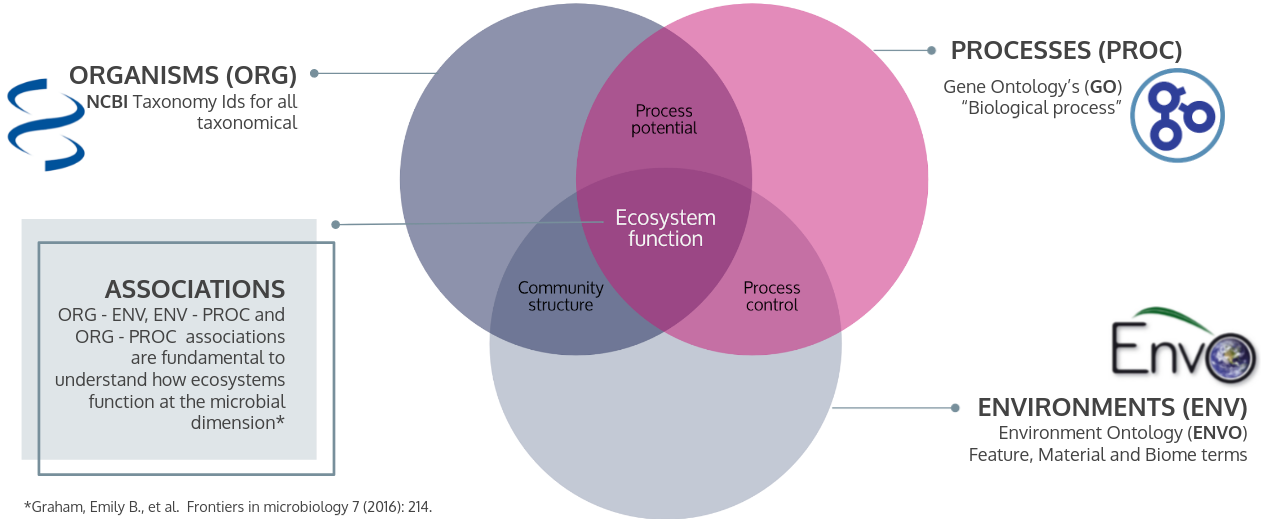
\includegraphics[width=105mm]{resources/prego_triple_associations.png}
   \end{frame}

   % METADATA
   \begin{frame}

      \frametitle{Metadata example}
      \framesubtitle{from various metagenome repositories}
      \begin{tikzpicture}[overlay,remember picture]
         \node[anchor=west, xshift=10pt, yshift=-5mm]
            at (current page.west) {
               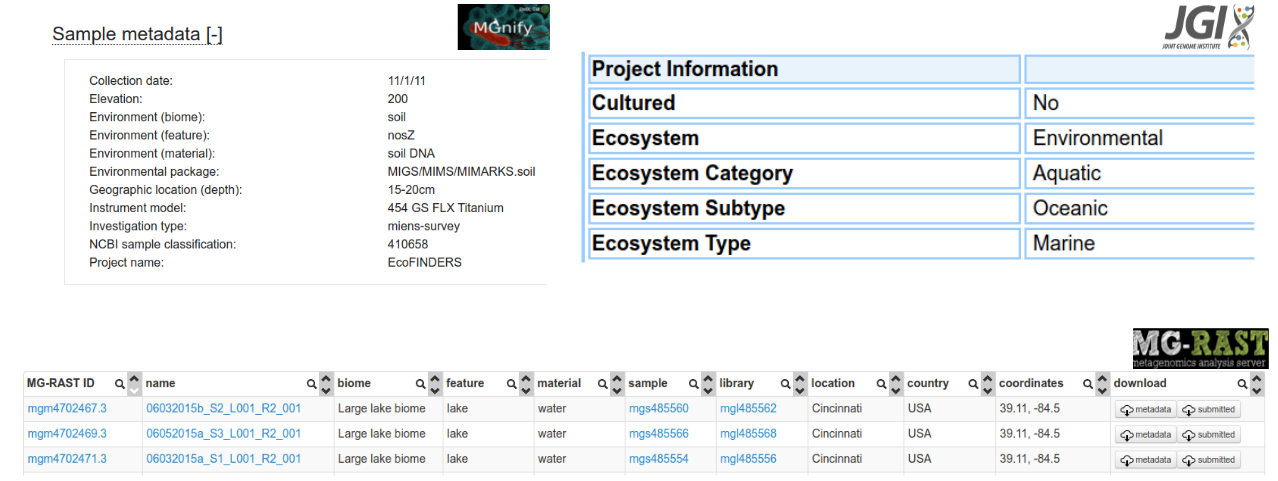
\includegraphics[width=120mm]{resources/metadata_like.png}
            };
         \end{tikzpicture} 
   \end{frame}

   % EXTRACT EXAMPLE
   \begin{frame}
      \frametitle{Named Entity Recognition}
      \framesubtitle{tagging the literature}
      \begin{figure}
         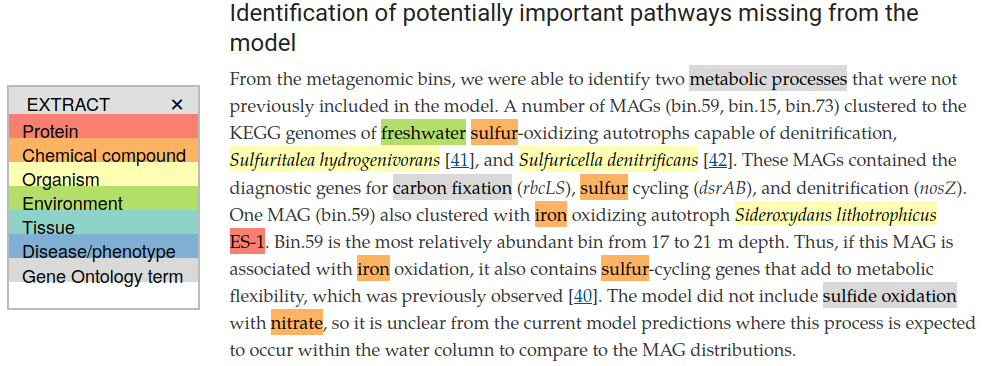
\includegraphics[width=105mm]{resources/extract_example_transp.png}
         \caption{
            \scriptsize Example text from Arora-Williams et al. Microbiome 6.1 (2018): 1-16.
         }
      \end{figure}
      
   \end{frame}

   % PREGO METHODOLOGY
   \begin{frame}

      \frametitle{PREGO methodology}
      \framesubtitle{co-occurrence again!}

      \begin{singlespace}
         \begin{tikzpicture}[overlay,remember picture]
            \node[anchor=north west, xshift=30pt,yshift=-70pt]
               at (current page.north west) {
                  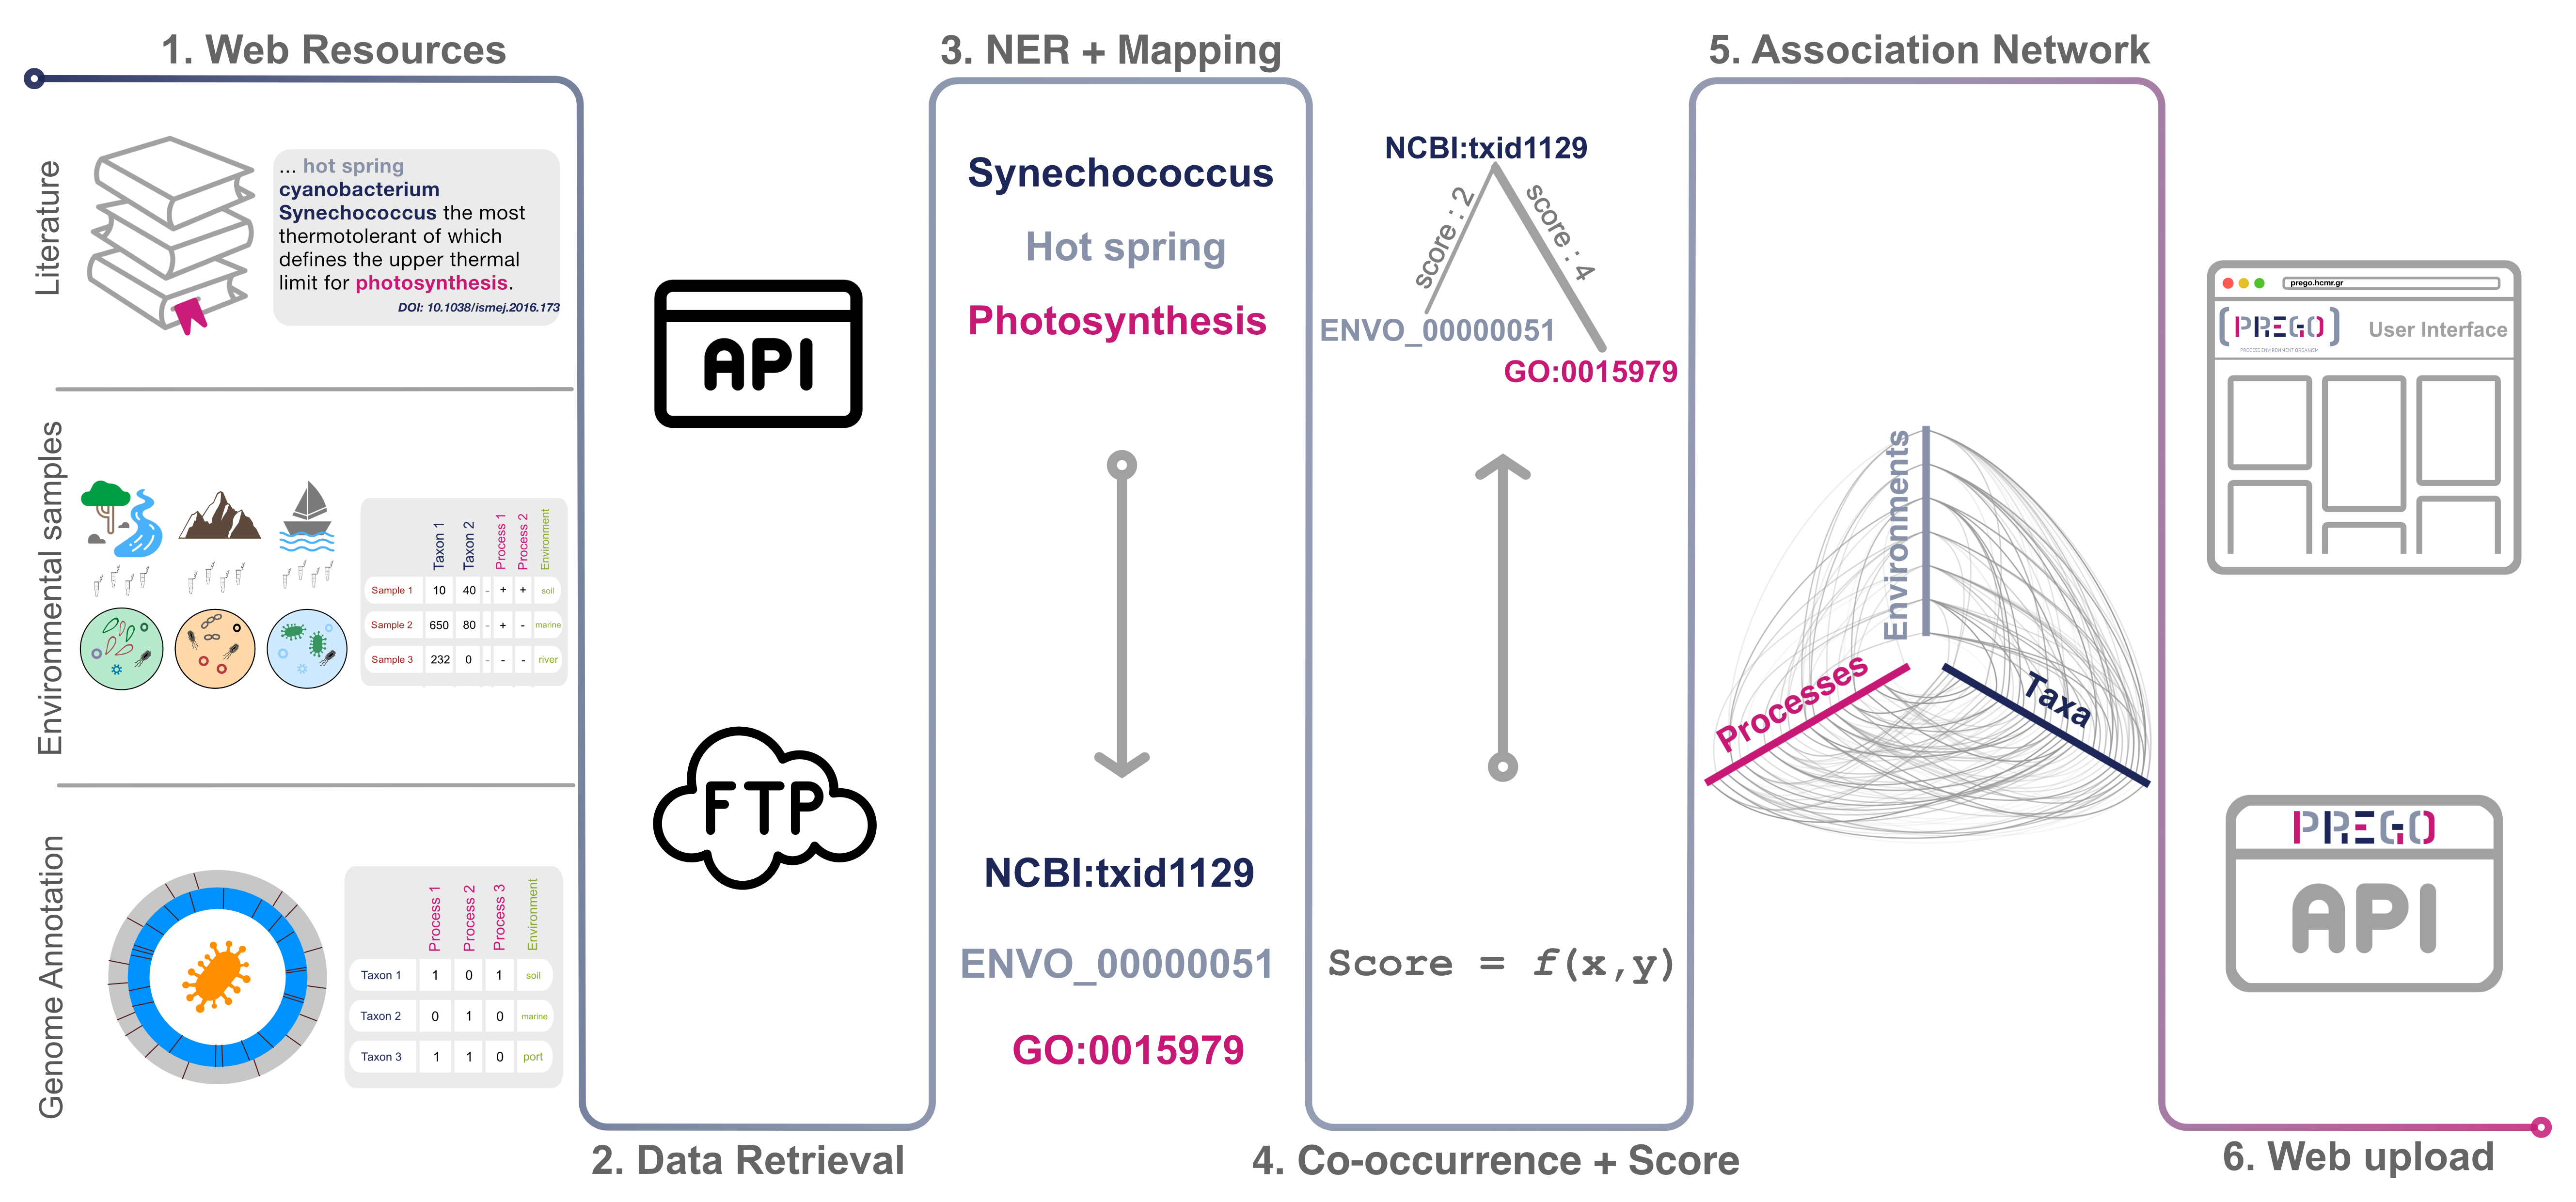
\includegraphics[width=105mm]{resources/figure_1_prego_analysis_horizontal_tr.png}
               };
            \node[align = left, above, yshift=30] at (current page.south) {
               \scriptsize 
               Figure from the PREGO publication that is now
               under review. 
               % at Special Issue  \\  
               % \scriptsize
               % "Selected Papers from the 9th Conference of the Hellenic Scientific Society MIKROBIOKOSMOS"
            };
         \end{tikzpicture}
      \end{singlespace}
   \end{frame}

   % DEVOPS
   \begin{frame}

      \frametitle{Building a knowledge-base}
      \framesubtitle{development and information technology operations}

      \begin{tikzpicture}[overlay,remember picture]
         \node[anchor=south west, xshift=10pt,yshift=30pt]
            at (current page.south west) {
               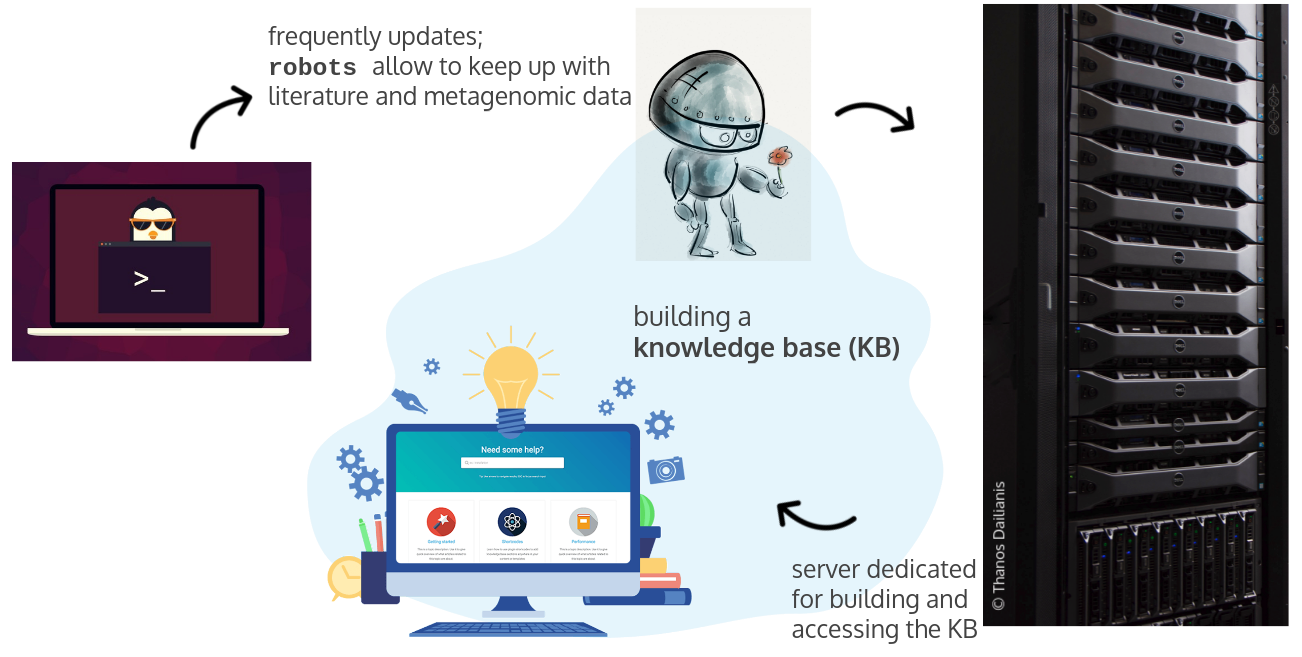
\includegraphics[width=120mm]{resources/prego_boots.png}
            };

            \node[anchor=south west, xshift=5pt,yshift=5pt]
            at (current page.south west) {
               
\includegraphics[width=35mm]{resources/devops.png}
            };
      \end{tikzpicture}
   \end{frame}


   % PREGO EXAMPLE
   \begin{frame}
      \frametitle{PREGO in action}
      \framesubtitle{looking for environments a taxon is present}

      \begin{tikzpicture}[overlay,remember picture]

         \node[anchor=west, xshift=5pt,yshift=10pt]
               at (current page.west) {
                  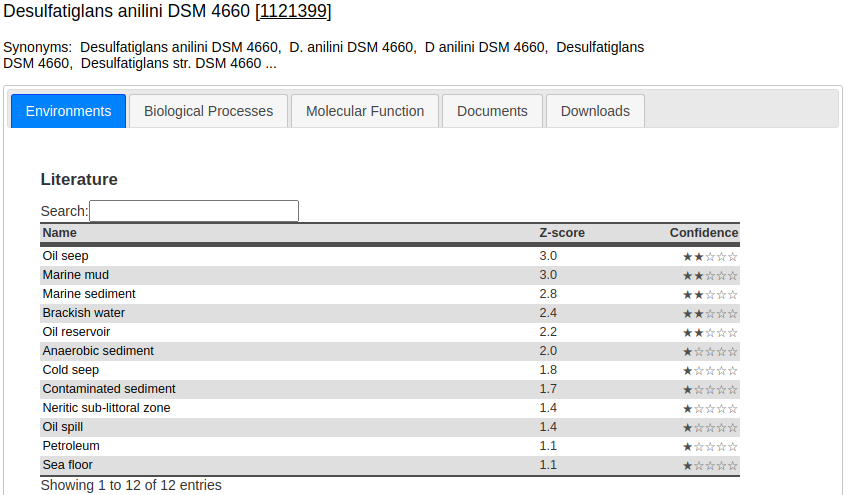
\includegraphics[width=63mm]{resources/prego_org_env_literature.png}
         };

         \node[anchor=east, xshift=-2pt,yshift=-25pt]
         at (current page.east) {
            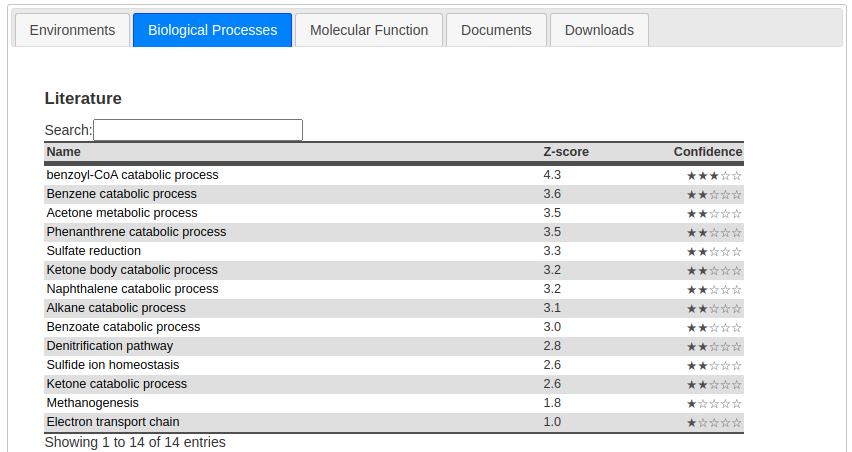
\includegraphics[width=65mm]{resources/prego_org_biol_proc_literature.png}
         };

      \end{tikzpicture}

   \end{frame}

   % -------------------------------------
   % CHANGE THE CHAPTER SLIDE: DINGO
   % -------------------------------------

   \begin{darkframes}
      \section{
         \texttt{dingo}: a Python library for metabolic flux sampling
      }   
   \end{darkframes}

   % DINGO LOGO - SLIDE
   \begin{frame}
      
      \begin{figure}
         
\includegraphics[width=55mm]{../met_nets/resources/dingo5_transparent.png}
      \end{figure}

      \begin{textblock*}{12cm}(3.5cm, 7cm)
         \href{https://github.com/GeomScale/dingo}{https://github.com/GeomScale/dingo}
      \end{textblock*}

   \end{frame}


   % % Sampling the flux space of microbial metabolic networks
   % \subsection{Flux sampling}

   % % BUILDIING MODELS
   % \begin{frame}{Genome-scale metabolic reconstruction}
      
   %    \begin{singlespace}
   %       \begin{tikzpicture}[overlay,remember picture]
   %          \node[anchor=north west, xshift=30pt,yshift=-50pt]
   %             at (current page.north west) {
   %                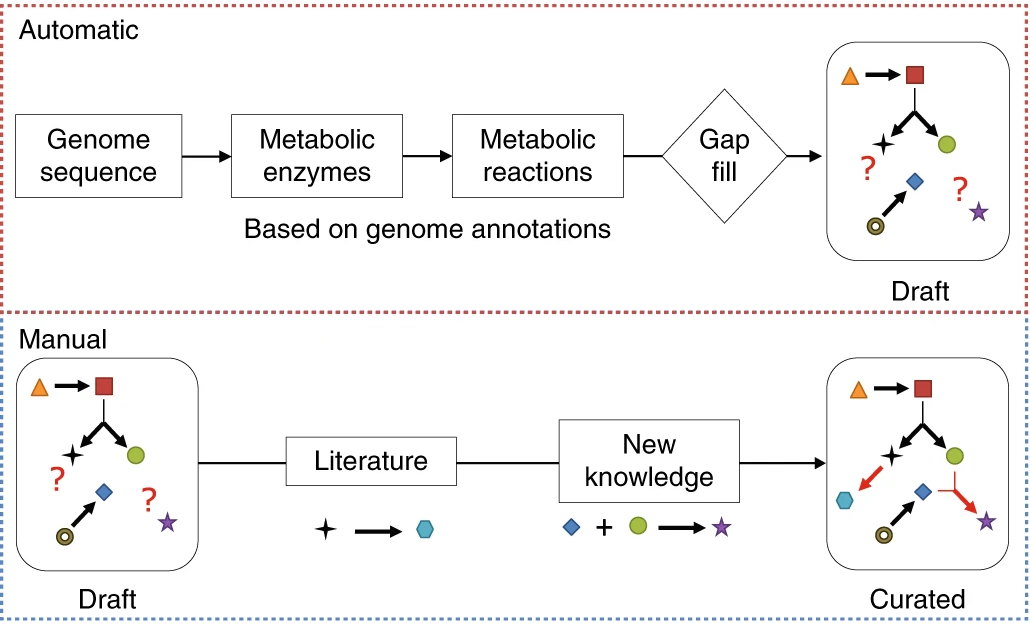
\includegraphics[width=105mm]{ ../met_nets/resources/building_gmd_transparent.png}
   %             };
   %          \node[align = left, above, yshift=10] at (current page.south) {
   %             \scriptsize 
   %             Figure from: Heirendt et al. Nature protocols 14.3 (2019): 639-702.
   %          };
   %       \end{tikzpicture}
   %    \end{singlespace}
   % \end{frame}
   
   % STOICHIOMETRIC MATRIX & FBA
   \begin{frame}{From a stoichiometric matrix}
      \framesubtitle{to a constraint-based model}
      
      \begin{singlespace}
         \begin{tikzpicture}[overlay,remember picture]

            \node[anchor=north west, xshift=20pt,yshift=-65pt]
               at (current page.north west) {
                  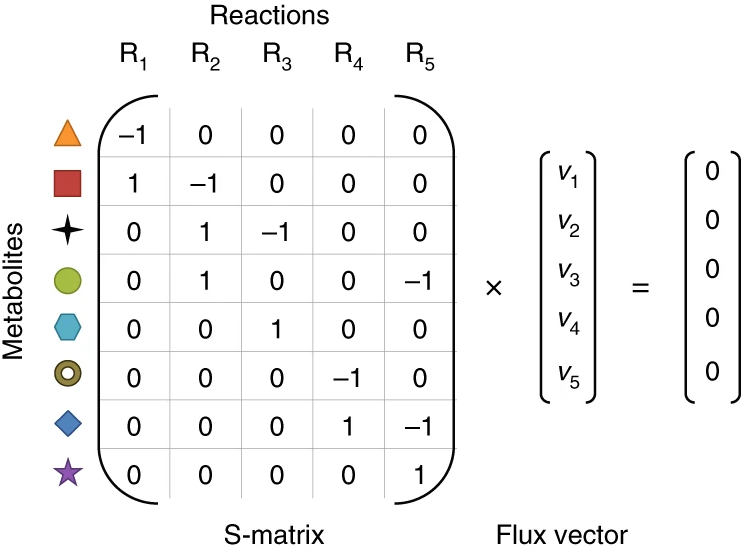
\includegraphics[width=70mm]{ ../met_nets/resources//stoichiometric_matrix_transparent.png}
               };

               \node[align = left, above, yshift=10] at (current page.south) {
                  \scriptsize 
                  Figure from: Heirendt et al. Nature protocols 14.3 (2019): 639-702.
               };
   
            \node[align = center, left, xshift=-10pt] at (current page.east) {
               \small
               \textbf{Flux Balance Analysis}
               \\ 
               \small
               Maximize \/ minimize an \\
               \small
               objective function:  \\
               \small
               $\psi = c_1 v_1 + c_2 v_2 + .. + c_5 v_5$ \\
               \small
               such that: \\
               \small
               $S * v = O$ \\ 
               \small
               and for each reaction $i$: \\
               \small
               $lb_i <= v_i <= ub_i$ \\ 
               
               \\

               \small
               where $lb$: lower bound, \\
               \small
               $ub$: upper bound and \\
               \small
               $S$: the stoichiometric matrix
            };

         \end{tikzpicture}
      \end{singlespace}      
   \end{frame}

   % FLUX SAMPLING
   \begin{frame}[label=simmonshall]{Flux sampling} 

      \framesubtitle{an alternative approach}
      \begin{singlespace}
         \begin{tikzpicture}[overlay,remember picture]

            \node[anchor=north west, xshift=30pt,yshift=-60pt]
               at (current page.north west) {
                  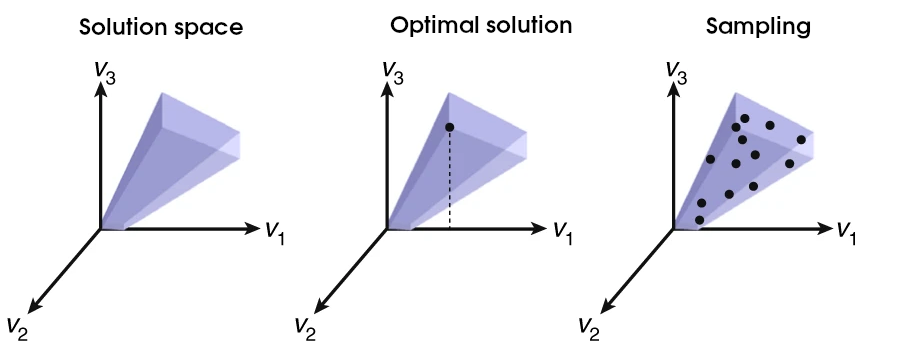
\includegraphics[width=100mm]{ ../met_nets/resources//solution_spaces_transparent.png}
               };

               \node[align = left, above, yshift=10] at (current page.south) {
                  \scriptsize 
                  Figure from: Heirendt et al. Nature protocols 14.3 (2019): 639-702.
               };

            \end{tikzpicture}

         \bigskip  \justifying  \bigskip
         \bigskip  \justifying  \bigskip
         \bigskip  \justifying  \bigskip

            \begin{itemize}
               \item \small 
               enables the analysis of GEMs without the need of an objective function
               \item \small
               determines the feasible solution spaces for fluxes in a network based on a set of conditions as well as the probability of obtaining a solution               
            \end{itemize}

      \end{singlespace}
   \end{frame}
 
   % MCMC ALGORITHM
   \begin{frame}{Our Markov Chain Monte Carlo (MCMC) algorithm}
      \framesubtitle{for flux sampling}

      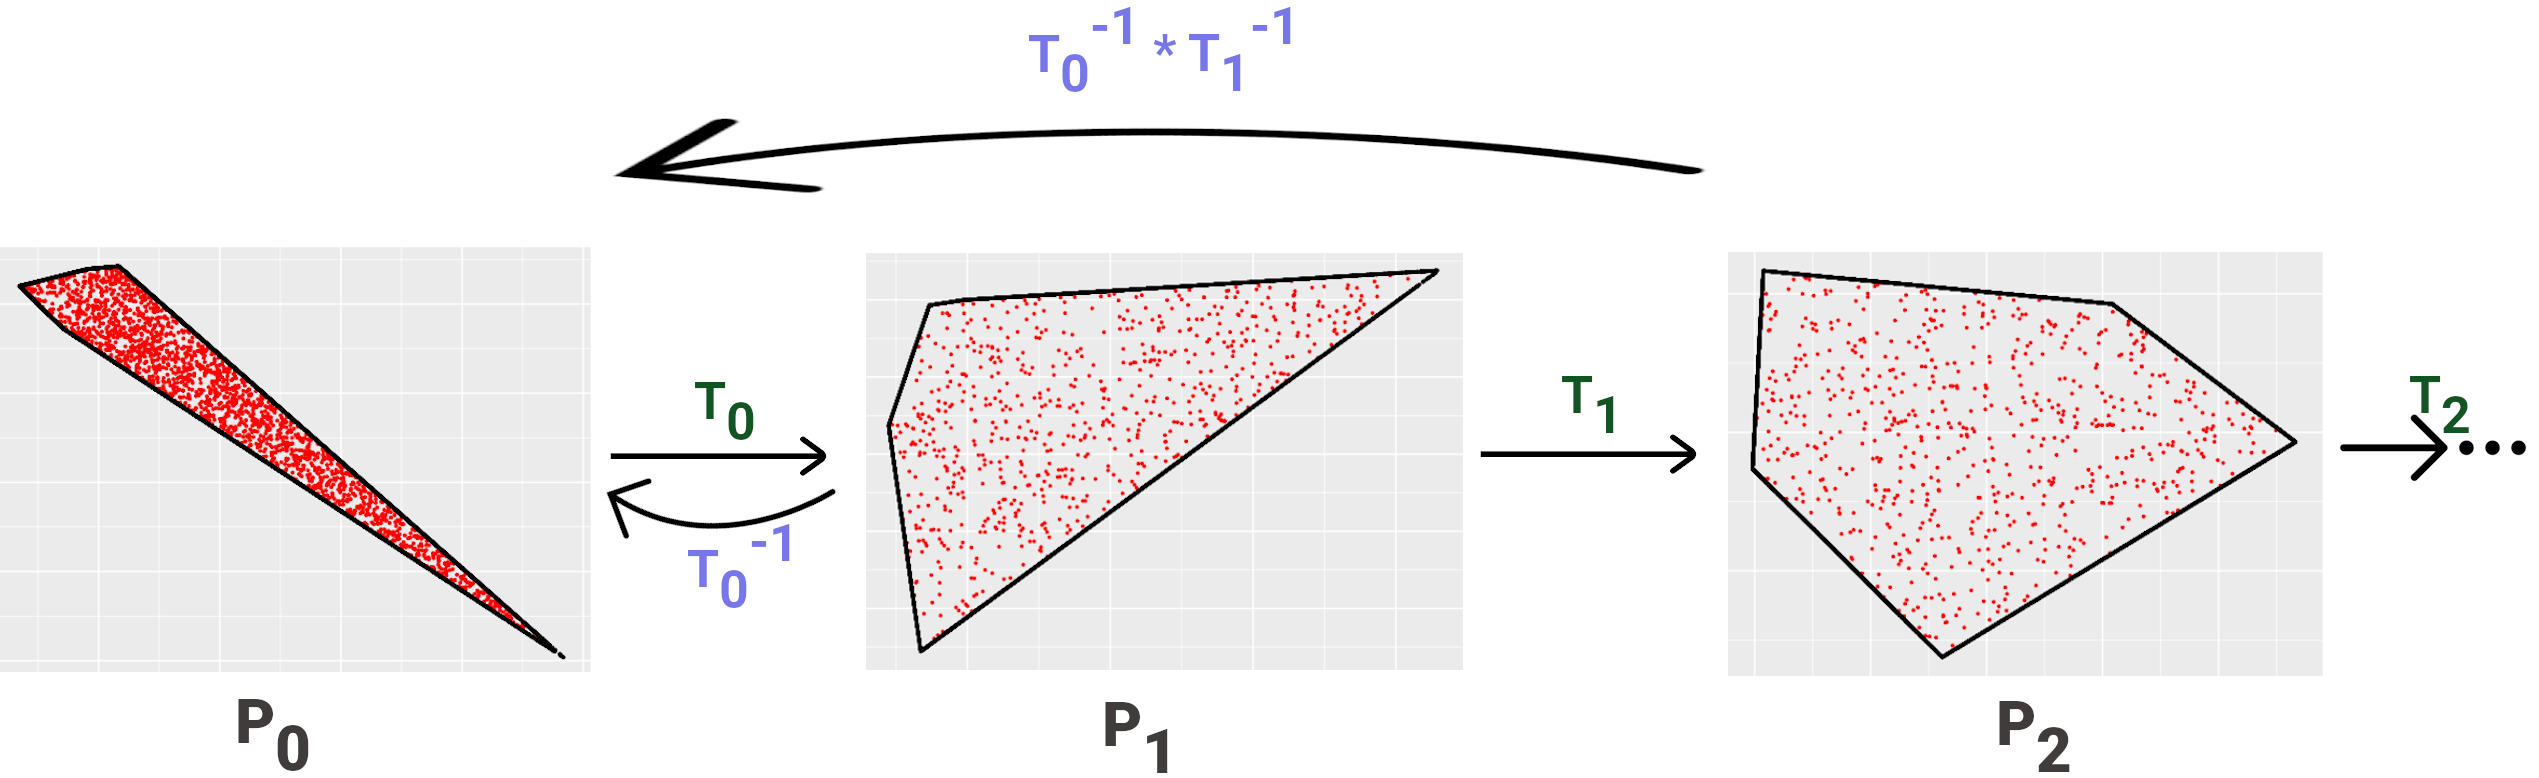
\includegraphics[scale=0.11]{ ../met_nets/resources//sampling_extra_phase_croped_transparent.png}
      
      \scriptsize
      \begin{block}{Steps of an MMCS phase}
         \begin{itemize}
            \item \textbf{sampling step:} using a variant of the \textbf{Billiard walk}  
            \item \textbf{rounding step:} calculate a linear transformation $T_i$ that puts the sample into isotropic position and then apply it on $P_i$ to obtain the polytope of the next phase
            \item check several statistic tests
         \end{itemize}      

      \end{block}

      % \begin{singlespace}
      %    \scriptsize
      %    Chalkis, Fisikopoulos, Tsigaridas and Zafeiropoulos 
      %    "Geometric Algorithms for Sampling \\ the Flux Space
      %    of Metabolic Networks", SoCG 2021,  
      %    DOI: 10.4230/LIPIcs.SoCG.2021.21
   
      % \end{singlespace}

   \end{frame}

   % RENZ ET AL. PAPER
   % \begin{frame}{Find possible targets against SARS-CoV-2}
   %    \framesubtitle{a flux sampling application}
   %    \bigskip
   %    
\includegraphics[scale=0.27]{ ../met_nets/resources//covid_paper.png}
      
   %    \begin{singlespace}
   %       \begin{itemize}
   %          \item \small Renz et al. '20 built the biomass function of Sars-Cov-2 to build a host - virus network
   %          \item \small Using FBA they computed an optimal steady state using \\ \small \quad (i) human biomass maintenance,\\ \small \quad (ii) virus growth rate
   %          \item \small They found reaction GK1 as a possible anti-viral target.
   %       \end{itemize}            
   %    \end{singlespace}

   % \end{frame}

   % SAMPLING ON THE RENZ ET AL. MODEL 
   \begin{frame}{Find possible targets against SARS-CoV-2}
      \framesubtitle{a flux sampling application}      

      \begin{tikzpicture}[overlay,remember picture]

         \node[anchor=north east, xshift=-10pt,yshift=-30pt]
            at (current page.north east) {
               
\includegraphics[width=20mm]{ ../met_nets/resources//dingo5_transparent.png}
            };
      \end{tikzpicture}


      \centerline{
      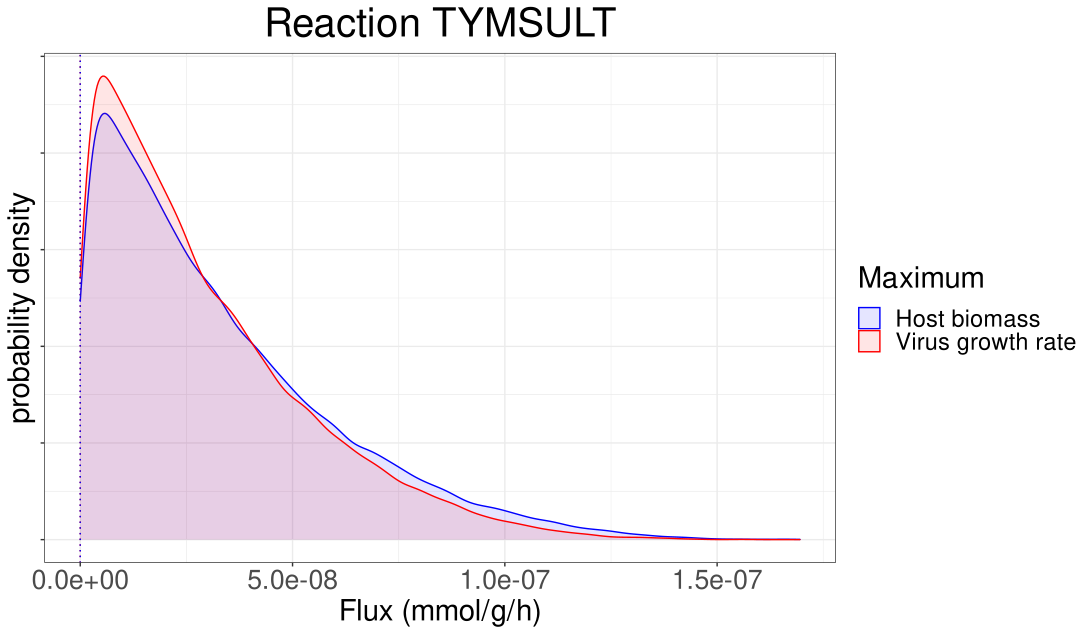
\includegraphics[scale=0.21]{
          ../met_nets/resources//density_flux_TYMSULT_fba_2_transparent
         } 
      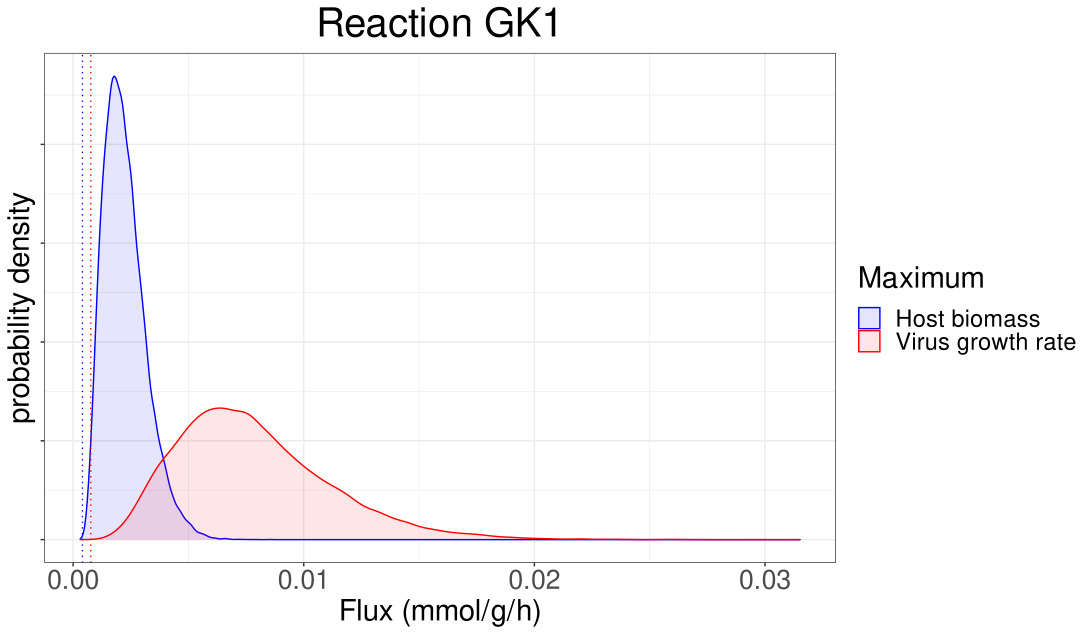
\includegraphics[scale=0.21]{
          ../met_nets/resources//density_flux_gk1_fba_2_transparent
         }
      }

      \begin{itemize}
         \item Check if the flux distribution of a reaction changes.
         \item Find possible anti-viral targets and study further.
      \end{itemize}
      \vspace*{0.2cm}

   \end{frame}
   
   % FLUX SAMPLING APPLICATIONS
   \begin{frame}{Further applications}
      \framesubtitle{of metabolic flux sampling}

      \begin{singlespace}

         \begin{columns}[onlytextwidth]

            \column{.5\textwidth}
               \begin{tikzpicture}[overlay,remember picture]
                  
                  \node[anchor=north west, xshift=15, yshift=-100pt]
                  at (current page.north west) {
                     
\includegraphics[width=55mm]{ ../met_nets/resources//cartoon_wine.jpg}

                  };

                  \node[align = left, above, xshift=-80, yshift=35] at (current page.south) {
                     \scriptsize Scott, William T., et al. "Metabolic flux sampling \\ 
                     \scriptsize predicts strain-dependent differences related to \\ 
                     \scriptsize 
                     aroma production among commercial wine yeasts." \\
                     \scriptsize
                      Microbial cell factories 20.1 (2021): 1-15.   
                  };
      
               \end{tikzpicture}



            \column{.5\textwidth}
               \begin{tikzpicture}[overlay,remember picture]

                  \node[anchor=north east, xshift=-45, yshift=-100pt]
                     at (current page.north east) {
                        
\includegraphics[width=30mm]{ ../met_nets/resources//interactions_transparent.png}
                     };

                  \node[align = right, above, xshift=95, yshift=65] at (current page.south) {
                     \small
                     What about microbial interactions ? 
                  };
                  % \node[align = right, above, xshift=-20, yshift=35] at (current page.south) {

                  %    fsfasfhasdf

                  % }

               \end{tikzpicture}
         \end{columns}
      \end{singlespace}
   \end{frame}

   % % dingo Python library
   % \begin{frame}{\texttt{dingo}: a Python library }
   %    \framesubtitle{for flux sampling}

   %    \begin{columns}[onlytextwidth]

   %       \column{.48\textwidth}
   %          
\includegraphics[scale=0.1]{ ../met_nets/resources//dingo5_transparent.png}
         
   %          \href{https://github.com/GeomScale/dingo}{https://github.com/GeomScale/dingo}

   %       \column{.41\textwidth}

   %          \begin{center}
   %             \texttt{how to} GCollab notebook
   %             
\includegraphics[scale=0.3]{ ../met_nets/resources//dingo_collab_transparent.png}               
   %          \end{center}
 
   %    \end{columns}

   % \end{frame}


   % -------------------------
   % CHANGE THE CHAPTER SLIDE: TRISTOMO SWAMP 
   % -------------------------
   % \begin{darkframes}
   %    \section{
   %       Tristomo swamp: a hybrid amplicon \& shotgun metagenomics analysis 
   %    }
   % \end{darkframes}


   % \begin{frame}
   %    \frametitle{A swamp in Karpathos}
   %    \framesubtitle{an Aegean island}
   %    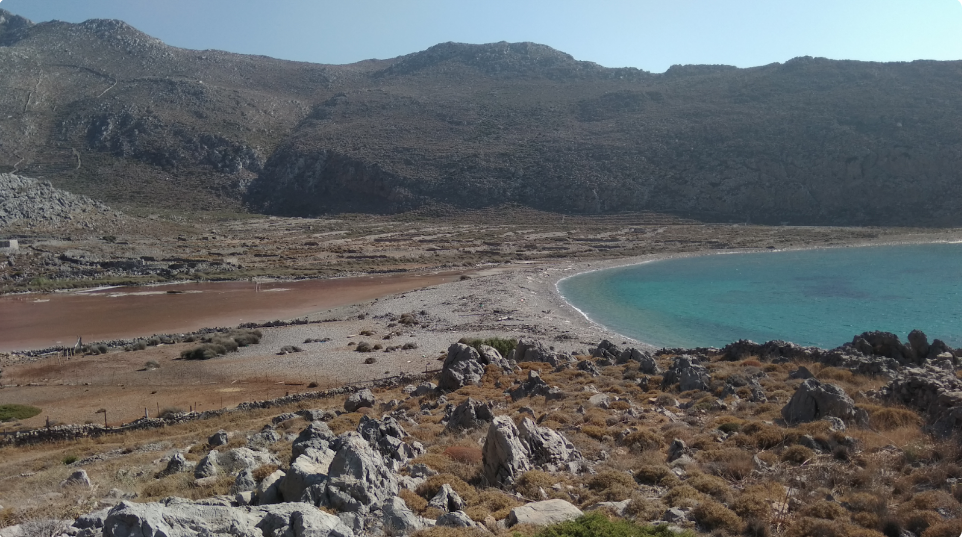
\includegraphics[width=85mm]{resources/tristomo_swamp.png}
   % \end{frame}


   % -------------------------------------
   % CHANGE THE CHAPTER SLIDE: HPC
   % -------------------------------------

   \begin{darkframes}
      \section{0s \& 1s in molecular biology}
   \end{darkframes}

   % ZORBAS PROJECT RESOURCES
   \begin{frame}

      \frametitle{Computational requirements}
      \framesubtitle{for \textit{trivial} bioinformatic tasks}

      \begin{tikzpicture}[overlay, remember picture]
         \node[anchor=north, yshift=-30mm]
            at (current page.north){
               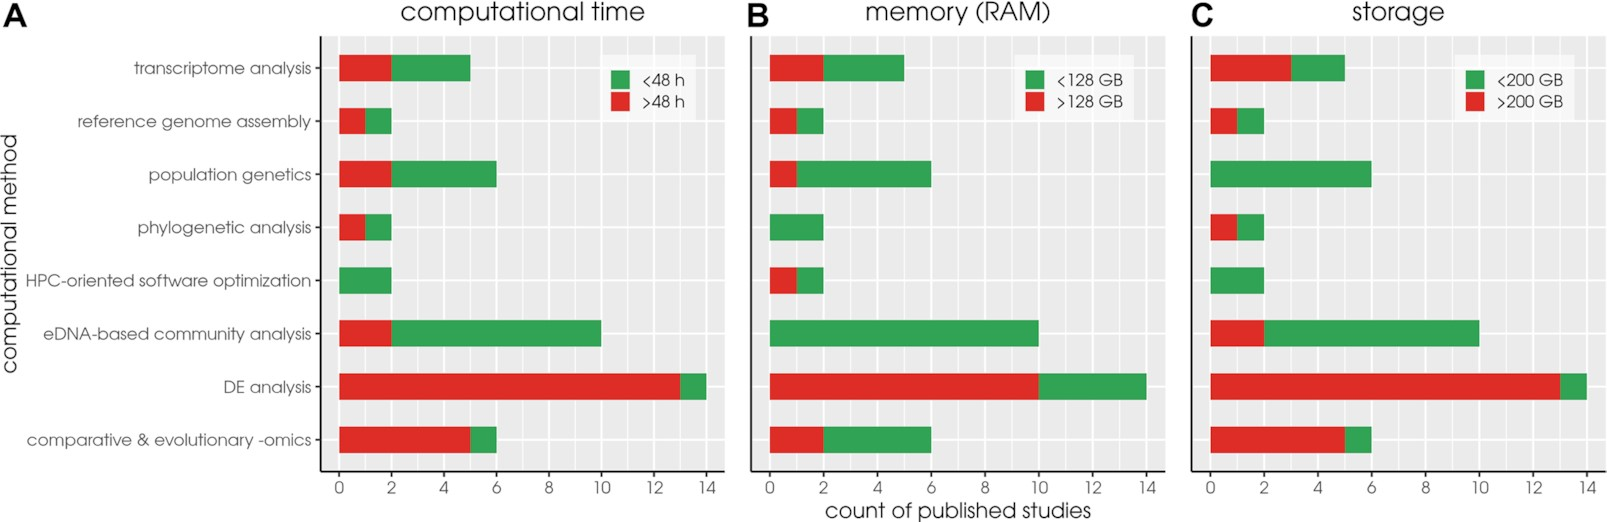
\includegraphics[width=105mm]{resources/imbbc_needs.jpeg}
            };
      \end{tikzpicture}

      \begin{textblock*}{10cm}(2cm, 7.5cm)
            \scriptsize Red bars denote published research with high resource requirements \\
            \scriptsize of the various computational methods employed at the IMBBC HPC facility
      \end{textblock*}


   \end{frame}

   % ZORBAS SCHEME
   \begin{frame}
   
      \frametitle{Zorbas: the HPC facility of IMBBC}
      \framesubtitle{a Tier 2 (regional) HPC facility}
      
      \begin{tikzpicture}[overlay, remember picture]
         \node[anchor=west, xshift=25pt, yshift=-20pt]
            at (current page.west){
               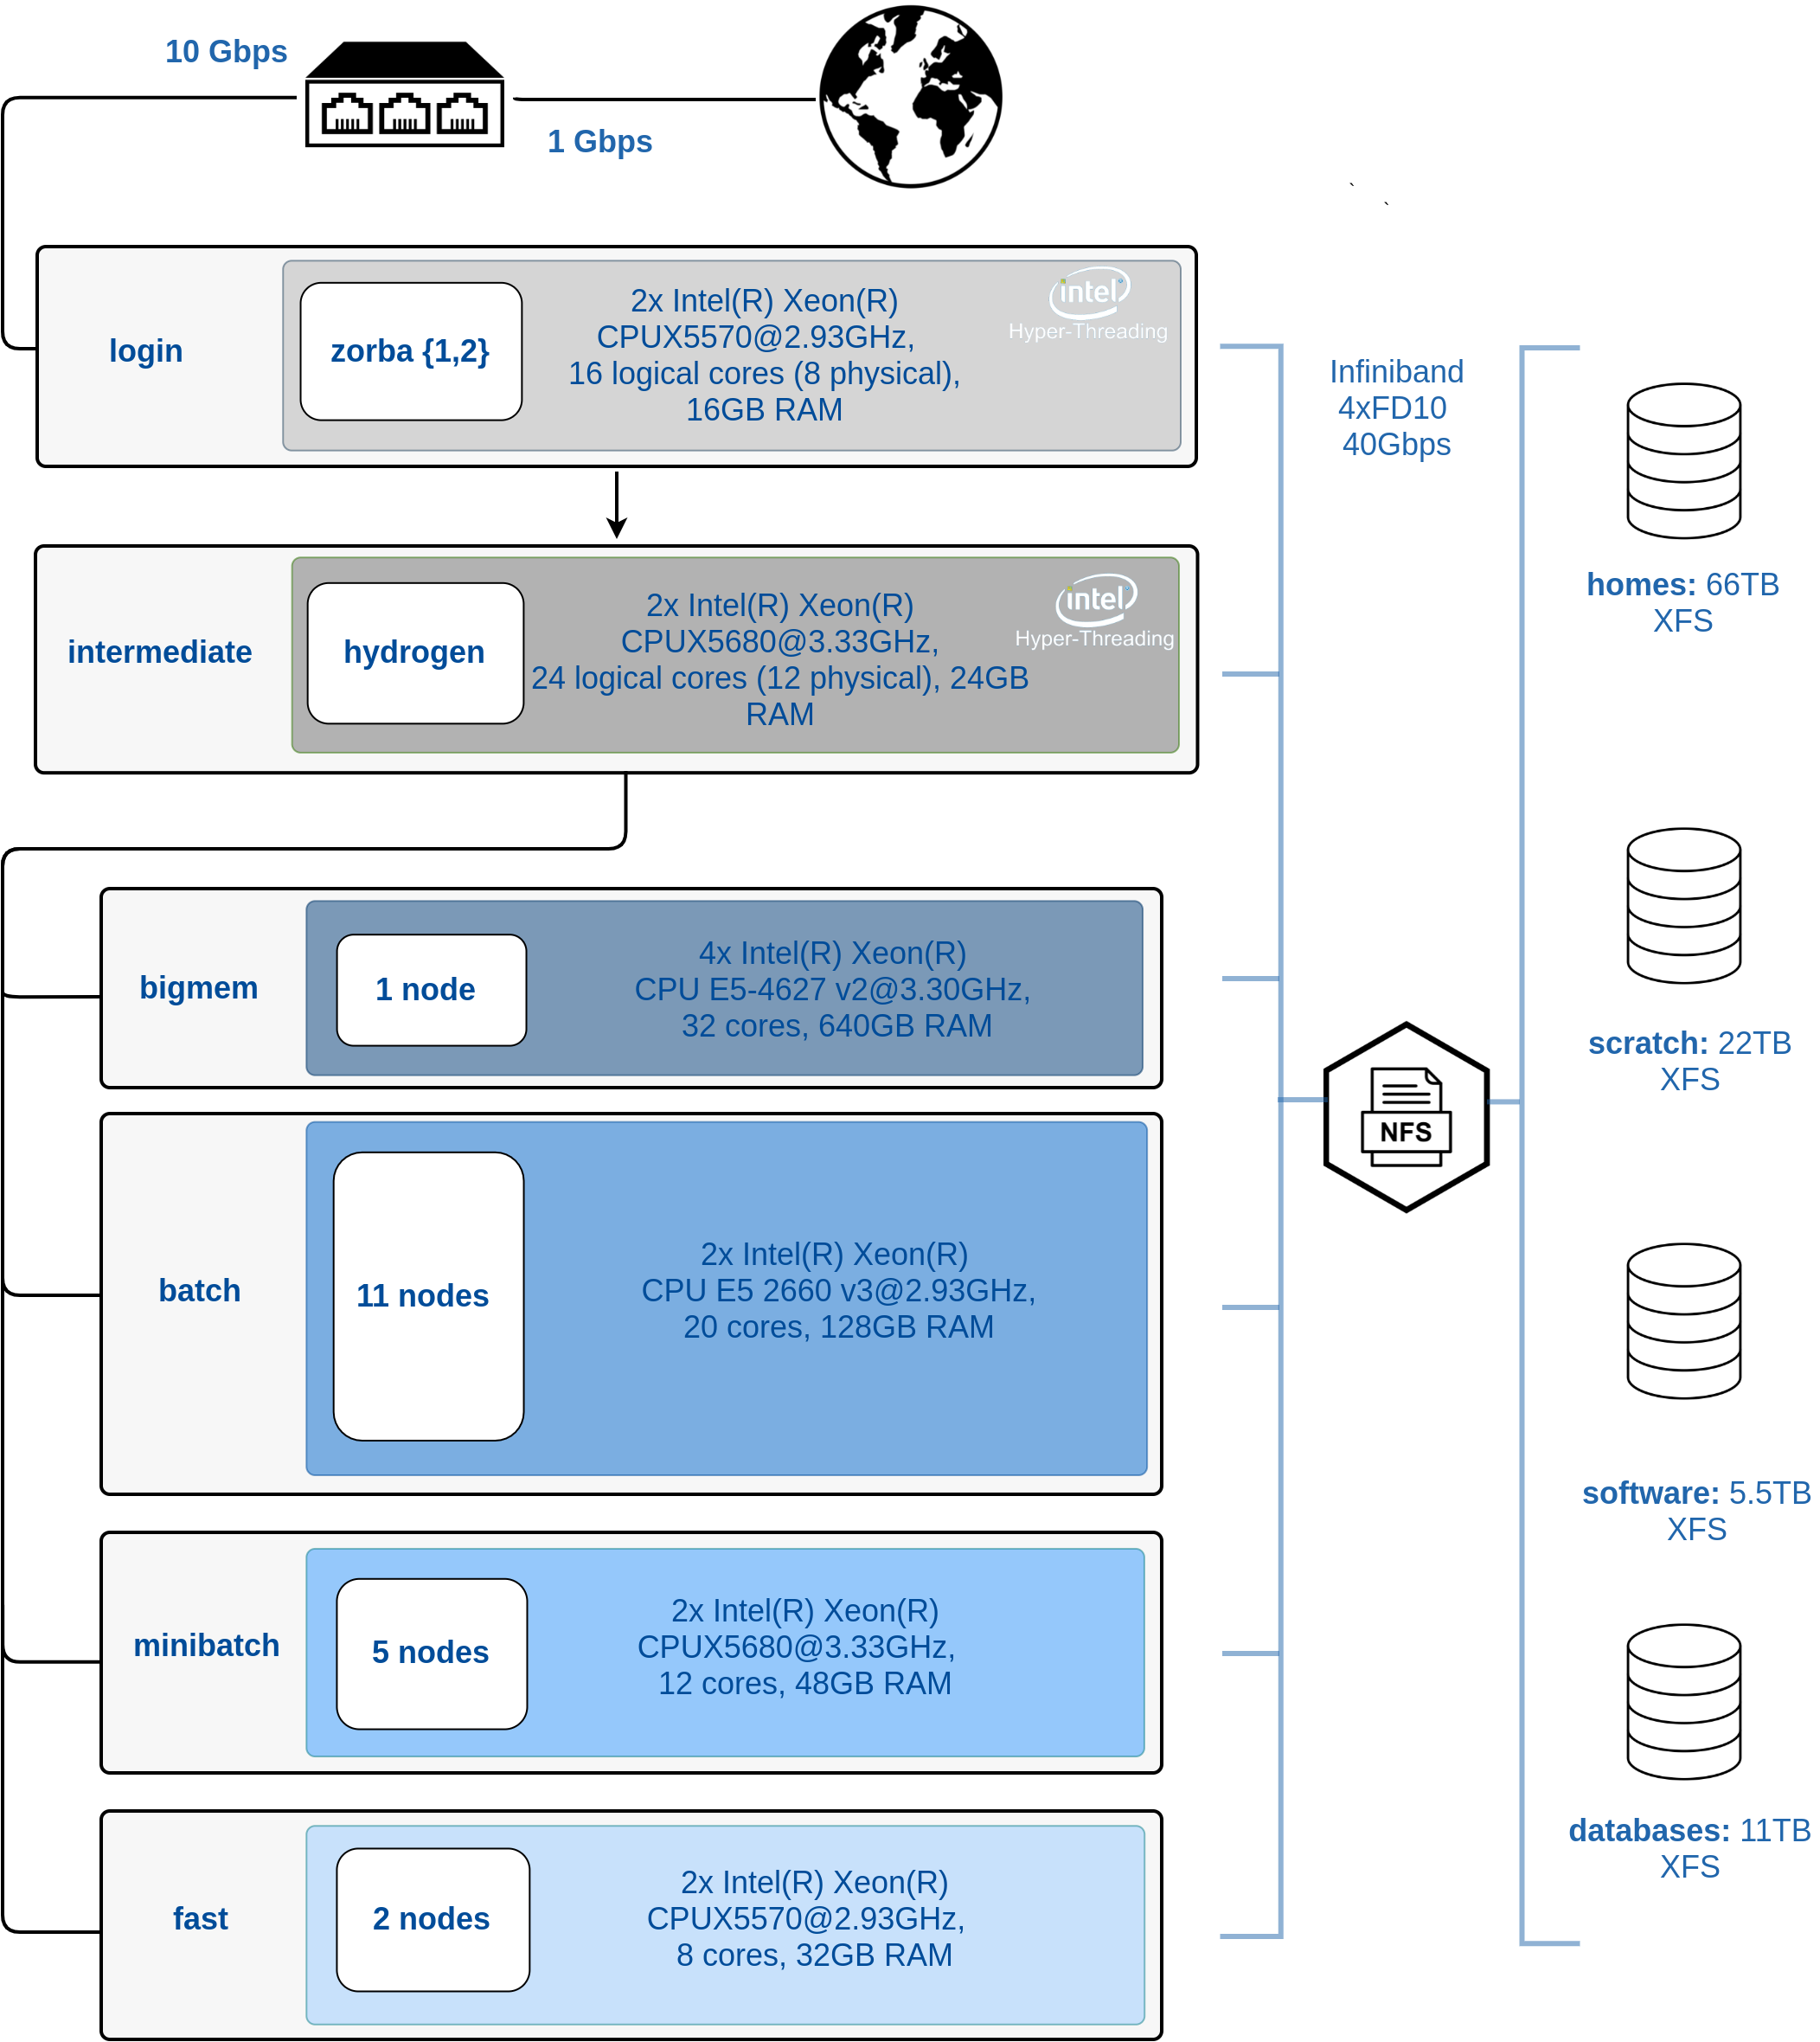
\includegraphics[width=60mm]{resources/zorbas_transp.png}
            };
         
      \end{tikzpicture}

      \begin{textblock*}{3.5cm}(8.5cm,5cm)
         Block diagram of the Zorba architecture
      \end{textblock*}
   
   \end{frame}

   % INFRASTUCTURES
   \begin{frame}
      \frametitle{Computing infrastructures}
      \framesubtitle{an alternative for the most!}
   
      \begin{tikzpicture}[overlay,remember picture]
         \node[anchor= west, xshift=10pt]
            at (current page.west){
               \includegraphics[width=60mm]{resources/marine-genomic-observatories.png}
            };
      \end{tikzpicture}


      \begin{textblock*}{5cm}(7.4cm, 3.0cm)

         \small We will develop a workflow  \\
         \small for the analysis of Genomic \\ 
         \small Observatories (GOs) data \\
         \small that will allow researchers \\ 
         \small to deal better with the  \\
         \small increasing amount of data

      \end{textblock*}
   
   \end{frame}

   % -------------------------------------
   % CHANGE THE CHAPTER SLIDE: MICROBETAG 
   % -------------------------------------
   \begin{darkframes}
      \section{
         \texttt{microbetag}: enhancing microbial interactions inference from co-occurrence networks
      }
   \end{darkframes}

   % MICROBETAG MODULES 
   \begin{frame}
      \frametitle{\texttt{microbetag}: annotating co-occurrence networks}
      \framesubtitle{a short term EMBO fellowship}

      \begin{textblock*}{5cm}(0.8cm, 3.5cm)
         Our short misssion consists of 3 modules: 
         
         \begin{itemize}
            \small \item pathway complementarity
            \small \item environmental conditions and phenotypic data integration
            \small \item flux sampling on pairs of metabolic models (if possible)
         \end{itemize}

      \end{textblock*}

      \begin{tikzpicture}[overlay,remember picture]
         \node[anchor=north east, xshift=-5pt,yshift=-55pt]
            at (current page.north east) {
               \includegraphics[width=62mm]{resources/Sources-of-co-occurrence-in-microbial-interaction-networks-A-Cooccurrence_W640_trans.png}
            };
         
      \end{tikzpicture}

      \begin{textblock*}{7cm}(6.0cm, 7.5cm)
         \scriptsize Figure from R{\"o}ttjers \& Faust (2018). 
                     FEMS microbiology reviews. 42. 10.1093/femsre/fuy030.
      \end{textblock*}


   \end{frame}

   % FIRST STEPS 
   \begin{frame}
      \frametitle{First steps}
      \framesubtitle{pathway complementarity}

      \begin{singlespace}
         
         \begin{textblock*}{10cm}(1.0cm, 2.7cm)
            
            \begin{enumerate}
               \small \item use abundance \& metadata table to run FlashWeave
               \small \item get the NCBI Taxon id of each taxon present in the edge file   
               \small \item search for available reference genomes for these ids 
               \small \item use KEGG modules to get major metabolic pathways of interest
               \small \item search for pathway complementarity in each module of interest
            \end{enumerate}

         \end{textblock*}

         \begin{textblock*}{10cm}(1.2cm, 6.0cm)

            \scriptsize Relative work \\ 
            \begin{itemize}
               \scriptsize \item \href{https://www.pnas.org/content/110/31/12804}{Levy \& Borenstein}. Proceedings of the National Academy of Sciences 110.31 (2013): 12804-12809. \\
               \scriptsize \item \href{https://www.pnas.org/content/112/20/6449.long}{Zelezniak et al.} Proceedings of the National Academy of Sciences 112.20 (2015): 6449-6454. 
            \end{itemize}
            
            
         \end{textblock*}



      \end{singlespace}

   \end{frame}

   % TOOLS AND DBs TO EXPLOIT
   \begin{frame}
      \frametitle{Databases to exploit}
      \framesubtitle{and how to}

      To get KO and further annotations of a taxon: 
      \begin{itemize}
         \item via KEGG organisms using \href{https://www.kegg.jp/kegg/rest/keggapi.html}{KEGG API}
         \item via JGI using the \href{https://github.com/ELIFE-ASU/ecg}{\texttt{ecg}} tool
         \item via BacDive using the \href{https://api.bacdive.dsmz.de/}{BacDive API} \\ 
         % client = bacdive.BacdiveClient('haris-zaf@hcmr.gr', 'k@r@vie@@k')
         % https://api.bacdive.dsmz.de/
         % https://pypi.org/project/bacdive/
         % to login there: https://api.bacdive.dsmz.de/login
      \end{itemize}

      Further annotation sources to be considered: 
      \begin{itemize}
         \item \href{https://pages.uoregon.edu/slouca/LoucaLab/archive/FAPROTAX/lib/php/index.php}{FAPROTAX}
         \item \href{https://bugbase.cs.umn.edu/}{BugBase}
         \item \href{https://bioinfo.imtech.res.in/manojk/sigmol/}{SigMol}
      \end{itemize}
      % \href{https://github.com/xuechunxu/DiTing}{https://github.com/xuechunxu/DiTing}

   \end{frame}

   % QUESTIONS TO BE ADDRESSED 
   \begin{frame}
      \frametitle{Open questions}
      \framesubtitle{just a few of them ;)  }

      \begin{itemize}
         
         \item species - strain inheritance in data integration
         \item dataset, maybe the \href{https://www.embopress.org/doi/full/10.15252/msb.20178157}{Venturelli} one 
         \item metabolic modelling at the community level
         \item competition and mutualism: a dialectic relationship
         
      \end{itemize}


   \end{frame}


   % -------------------------
   % PUBLICATIONS
   % -------------------------
   \begin{darkframes}
      \section{Publications}
   \end{darkframes}

   % PUBLICATIONS FRAME
   \begin{frame}[label=bibliography]{Publications}
      \framesubtitle{\TeX, \LaTeX, and Beamer}
      \begin{thebibliography}{9}

         \scriptsize
         \bibitem{prego}
            Zafeiropoulos, H., Paragkamian, S., Ninidakis, S., Pavlopoulos, G.A., Jensen, L.J. \& Pafilis, E. PREGO: a literature- and data-mining resource to associate microorganisms, biological processes, and environment types. - \textbf{\textit{under review}}


         \scriptsize
         \bibitem{darn2021}
            Zafeiropoulos, H., Gargan, L., Hintikka, S., Pavloudi, C., \& Carlsson, J. (2021). The Dark mAtteR iNvestigator (DARN) tool: getting to know the known unknowns in COI amplicon data. \href{https://mbmg.pensoft.net/article/69657/list/9/}{Metabarcoding and Metagenomics, 5, e69657.}
         \scriptsize

         \bibitem{mmcs2021}
            Chalkis, A., Fisikopoulos, V., Tsigaridas, E., \& Zafeiropoulos, H. (2021). Geometric algorithms for sampling the flux space of metabolic networks, \href{ https://drops.dagstuhl.de/opus/volltexte/2021/13820/}{37th International Symposium on Computational Geometry (SoCG 2021).}

         \scriptsize
         \bibitem{hpc2021}             
            Zafeiropoulos, H., Gioti, A., Ninidakis, S., Potirakis, A., Paragkamian, S., ... \& Pafilis, E. (2021). 0s and 1s in marine molecular research: a regional HPC perspective. \href{https://academic.oup.com/gigascience/article/10/8/giab053/6353916}{GigaScience, 10(8), giab053.}

         \scriptsize
         \bibitem{pema2020}
            Zafeiropoulos, H., Viet, H. Q., Vasileiadou, K., Potirakis, A., Arvanitidis, C., Topalis, P., ... \& Pafilis, E. (2020). PEMA: a flexible Pipeline for Environmental DNA Metabarcoding Analysis of the 16S/18S ribosomal RNA, ITS, and COI marker genes. \href{https://academic.oup.com/gigascience/article/9/3/giaa022/5803335}{GigaScience, 9(3), giaa022.}
 
      \end{thebibliography}
   \end{frame}

   % Thank you SLIDE
   \begin{darkframes}
   \begin{frame}{Thank you for your attention}

      \framesubtitle{and your patience ;)}
      % URLs
      GitHub   : \href{https://github.com/hariszaf}{https://github.com/hariszaf} \\
      email    : \href{haris-zaf@hcmr.gr}{haris-zaf@hcmr.gr} \\
      Twitter  : \href{https://twitter.com/haris_zaf}{haris\_zaf} \\
      web-site : \url{https://hariszaf.github.io/} \\
      

      \begin{textblock*}{4.0cm}(10.0cm, 2.5cm)

         \scriptsize \textbf{Spacial thanks to:} \\

         \scriptsize \href{http://lab42open.hcmr.gr/people/evangelospafilis/}{Dr. Pafilis E.} \\
         \scriptsize \href{https://cpavloud.github.io/mysite/projects/}{Dr. Pavloudi C.} \\ 
         \scriptsize \href{https://imbbc.hcmr.gr/user/s-paragkamian/}{PhD Paragkamian S.} \\
         \scriptsize \href{https://tolischal.github.io/}{Dr. Chalkis A.} \\
         \scriptsize \href{https://who.paris.inria.fr/Elias.Tsigaridas/}{Prof. Tsigaridas E.} \\
         \scriptsize \href{https://vissarion.github.io/}{Dr. Fisikopoulos V.} 
         
      \end{textblock*}

      % Logos   
      % -------------- 

      % UoC
      \begin{tikzpicture}[overlay,remember picture]
         \node[anchor=south west,
               xshift=-350pt,
               yshift=10pt]
               at (current page.south east) {
                  \includegraphics[height=17mm]{
                      ../met_nets/resources//UoC_logo_white.png
                  }
               };
      \end{tikzpicture}

      % IMBBC
      \begin{tikzpicture}[overlay,remember picture]
         \node[anchor=south east,
            xshift=-185pt,
            yshift=25pt]
            at (current page.south east) {
               \includegraphics[width=35mm]{ ../met_nets/resources//logo-imbbc.png}
            };
      \end{tikzpicture}%

      % HCMR
      \begin{tikzpicture}[overlay,remember picture]
         \node[anchor=south east,
               xshift=-125pt,
               yshift=10pt]
               at (current page.south east) {
                  \includegraphics[height=20mm]{
                      ../met_nets/resources//hcmr-logo.png
                  }
               };
      \end{tikzpicture}

      % GeomScale
      \begin{tikzpicture}[overlay,remember picture]
         \node[anchor=south east,
               xshift=-5pt,
               yshift=22pt]
               at (current page.south east) {
                  \includegraphics[width=40mm]{
                      ../met_nets/resources//geomscale-logo.png
                  }
               };

      \end{tikzpicture}

      % EMBO 
      \begin{tikzpicture}[overlay, remember picture]
         \node[anchor=south east, xshift=-10pt, yshift=75pt]
            at (current page.south east){
               \includegraphics[width=25mm]{resources/embo_logo_white.png}
            };
         
      \end{tikzpicture}



   \end{frame}
   \end{darkframes}

\end{document}
